% !TEX root = ./dissertation.tex
% !TEX TS-program = pdflatex
% !TEX encoding = UTF-8 Unicode
% !TEX spellcheck = en-US
% !BIB TS-program = = biber
\documentclass[twoside,11pt,american,openright,final]{memoir}
% Documentclass options:
% "draft" for draft mode (quicker build)
% "showtrims" to show trimmed sides before printing
\usepackage{SSEThesisPreamble}
\usepackage{pdfpages}

\title{Modeling Retail Performance Through Customer Behavior}
\newcommand\thesubtitle{Evidence from Multiformat, Multichannel, and Platform Settings}
\author{Tanetpong~(Ned)~Choungprayoon} % Use ~ instead of space to prevent line breaking

% Load the layout
\usepackage{SSEThesisLayout}

% All included chapters need to have their graphics paths specified manually here
% this is for input to work and to find the right figures
% Graphics paths for all documents
\graphicspath{{./chapters/figures/}{./chapters/chapter2/figures/}}
\makeatletter
\providecommand*{\input@path}{}
\g@addto@macro\input@path{{./chapters/chapter1/figures/}{./chapters/chapter2/figures/}}%
\makeatother

% Bibliographies (can be multiple files)
\addbibresource{chapters/bibliography.bib}

\begin{document}
\frontmatter
\thispagestyle{empty}

%%%%%%%%%%%%%%%%
% TITLE PAGE (right side)
\vspace*{4\onelineskip}
\begin{center}
{\Huge\sffamily\thetitle}\par\vspace*{2\onelineskip}
{\Large\sffamily\thesubtitle}\par\vspace*{2\onelineskip}
{\Large\sffamily\theauthor}\par
\end{center}

\vfill

\begin{center}

\includegraphics[width=2.88cm]{logo_black.pdf}
\end{center}

\pagebreak

%%%%%%%%%%%%%%%%
% Copyright page (on left side)
\thispagestyle{empty}
\begin{flushleft}
\begin{tabularx}{\textwidth}[t]{m{1.93cm}X}

\includegraphics[width=1.93cm]{logo_black} &
\begin{tabular}{@{}l@{}}
	Dissertation for the Degree of Doctor of Philosophy, Ph.D.,\\
	in Business Administration\\
	Stockholm School of Economics, 2026\\
\end{tabular}\\
\end{tabularx}
\vfill
\thetitle : \thesubtitle\par
\textcopyright~\theauthor, 2026\par\bigskip
ISBN 978-91-7731-405-9 (printed)\par
ISBN 978-91-7731-406-6 (pdf)\par\bigskip
This book was typeset by the author using \LaTeX.\par\bigskip
\emph{Front cover photo}: \textcopyright~Neddie~\&~Riety,~2026\par\bigskip
\emph{Back cover photo}:~Juliana~Wolf~Garcindo,~2019\par\bigskip
\emph{Printed by}: Universitetsservice US-AB, Stockholm, 2026\par\bigskip
\emph{Keywords:} Store formats, Multichannel, Grocery Retailing, Music Streaming, Digital Platform, Pricing, Discounts, Customer Category Purchase, Private labels, Online Adoption, Retailer revenue, Playlist Followers,  Pandemic
\end{flushleft}

% Dedication
\cleardoublepage
\thispagestyle{empty}
\vspace*{45mm}
\begin{center}
\textit{To}

\textit{My Family}

\textit{And My Beloved Friends,}

\textit{Both Those I Have Met and Those I Have Yet to Meet}
\end{center}

\cleardoublepage
%%%%%%%%%%%%%%%%%%
% Foreword
\chapter*{Foreword}\thispagestyle{empty}
This volume is the result of a research project carried out at the Department of Marketing and Strategy at the Stockholm School of Economics (SSE).

This volume is submitted as a doctoral thesis at SSE. In keeping with the policies of SSE, the author has been entirely free to conduct and present his research in the manner of his choosing as an expression of his own ideas.

SSE is grateful for the financial support provided by Torsten Söderbergs Stiftelse, Ann-Margret och Bengt Fabian Svartz Stiftelse, and Hans Werthénfonden, which has made it possible to carry out the project.

\vspace{2\onelineskip}

\begin{tabular}{cc}
\emph{Göran Lindqvist} & \emph{Hans Kjellberg}\\
& \\
Director of Research & Professor and Head of the\\
Stockholm School of Economics & Department of Marketing and Strategy\\
\end{tabular}
\cleardoublepage

%%%%%%%%%%%%%%%%%%%%%%%%%%%%%%%%%%%%%%%%%%%%%%%%%%%%%%%%%%%%%%%%%%%%%%%%%%%%%%%%%%%%%%%
% Preface

\chapter*{Preface}
\markboth{Preface}{}
% lägg in titlar

Let’s be honest: chances are you’re not going to read this entire thesis, and that’s totally fine. You’re probably here because this is the preface and it’s the perfect place to begin (and perhaps to end). We are all busy, right? Academics are busy working on papers (publish or perish!), and practitioners are swamped with back-to-back meetings and projects. But stick with me for just this short prologue.

Over the past five years, my PhD has kept me deeply interested in retail analytics. The questions I ask might sound familiar (as some might say, not particularly groundbreaking): Why do discounts work better in some stores than others? How does launching an online channel shift customer behavior?\footnote{Throughout this thesis, the terms consumer and customer are used with distinct but related meanings. The term consumer refers to general consumer behavior, particularly the psychological and decision-making processes often examined in consumer behavior research. The main focus of this thesis is on customers, taken as individuals actively interacting with retailers within the studied empirical settings. In other words, this thesis draws on consumer theory to explain how retailers might expect their customers to respond to strategic actions} What happens to customer behavior on digital platforms in the face of an external shock like COVID-19? These are questions that retailers, like consumers, ask all the time. What sets this work apart is my ability (and privilege) to spend half a decade or more exploring the questions with solid data, structured models, and consumer behavior theory to help connect the dots between observed patterns and strategic outcomes.
In this thesis, I look at how retailers adapt their pricing, channel, and platform strategies, and I examine how customers respond in ways that impact sales, profits, and outcomes on digital platforms. With the help of data and theory, I try to figure out what works, where, and why.
Here’s what you’ll discover.


\textbf{1. Multiformat: Pricing Strategy and Store Contexts}

Choosing a price is one thing, but it is another thing to know how customers respond differently to that price depending on where they shop. In the first two of the studies presented herein, I examine how pricing affects customer behavior across different physical store formats including hypermarkets, supermarkets, and convenience stores. The first study looks at private label tiers. Including basic, standard, and premium tiers, it shows that sales and profit elasticity vary significantly depending on the store format. The second study compares regular price reductions with promotional price discount. It shows that the same price cut can produce different effects depending on the context.

\textbf{2. Multichannel: The Long-Term Impact of Going Online}

In the third study, I investigate how online channel adoption changes customer behavior over the long run. The study finds that online adoption leads to long-term changes: larger basket sizes, increased spending in bulky or heavy categories like bottled water, and reduced purchases in impulse-driven or perishable items like snacks or fresh vegetables. These shifts reflect stable changes in how customers allocate effort and convenience across channels. Rather than cannibalizing in-store sales, online channels can enhance overall customer value.

\textbf{3. Platform: Customer Behavior During External Shocks}

In the final study, I examine how customer behavior on digital platforms shifted during the COVID-19 pandemic. The study uses follower growth on Spotify playlists as an empirical example to capture changes in this digital platform context. The results show that playlists curated by the platform remained resilient, but those associated with major record labels and superstar tracks lost momentum. The takeaway addresses more than music. In algorithmic environments where attention is scarce, resilience comes from diversified offerings, mid-tail strategies, and institutional curation, not from a sole product’s power or influence. For retailers operating on digital platforms, this highlights the importance (especially during periods of uncertainty) of visibility management and content strategy.

If you continue flipping through the pages of this thesis, you will come across theoretical discussions, mathematical notations, and statistical models. Such material might not be everyone’s cup of tea, but that is what academics thrive on: building on past research, applying theories to explain real-world phenomena, and using mathematical formulas as precision tools to quantify observations and draw conclusions. Don’t worry; the theoretical discussions and equations are here to shed light on how retail strategies, in pricing and platforms, connect with customer behavior. It is like building a house, where theory provides the blueprint, data supplies the raw materials, and models are the tools that assemble everything into something meaningful and durable.

This thesis is not a definitive guide to retail strategy. What I offer is a series of observations, tests, and tentative conclusions grounded in empirical data. The value is not just in the answers but in the act of asking, of looking closely, questioning assumptions, explaining patterns. I hope to show that doing research is less about undeniable truths and more about honest attempts. Attempts to understand, to explain, to make sense of a world that is constantly shifting, sometimes so dramatically that it breaks whatever model was in development. And in the end, maybe that’s the real strategy: stay curious, stay skeptical, and never trust a finding that required three robustness checks and a prayer.


%(\cite{Altmejd2018_predicting_replicability})


%\bigskip\fancybreak{{* * *}}\bigskip

%Some more really great text about the second paper, based on %\textcite{Camerer2016_evaluating_replicability}.

\cleardoublepage

%%%%%%%%%%%%%%%%%%
% Acknowledgements
\cleardoublepage
\chapter*{Acknowledgements}
\markboth{Acknowledgements}{}
\thispagestyle{empty}
%\pagestyle{empty}

I have far more people to thank than these pages can reasonably accommodate. In fact, I could probably write another thesis just for that. But in the interest of keeping things readable, I will focus here on a few individuals and groups, while many others are acknowledged throughout without being named individually. If you are reading this, you will likely know where you belong. And if I read this again in fifty years, I may forget some names, but not the memories.

Finally, this is coming to an end. First, I would like to thank myself for being patient and perseverant enough to drag this across the finish line. To my parents, mom and dad, thank you for the constant reminder that you were fully prepared to fly over and make sure I finished this PhD one way or another. Your unwavering support, both financial and otherwise, made it possible for me to pursue this path while somehow maintaining a lifestyle that suggests I made better financial decisions than I actually did. You made it possible for me to pursue a PhD full-time, even though at this stage of life, a stable corporate career would have been the more expected path in our culture. And to my brother, thank you for providing just enough early-life motivation to keep me moving forward.

To my “SSE academic family”: Sara Rosengren, for being the kind of mentor who gently but persistently pushes things to completion. I still remember sitting with you going line by line, brand by brand, category by category through grocery retail data until things finally started to make sense. Rickard Sandberg, for being supportive, understanding, and for always saying yes, especially to my reimbursement requests. With you, it was R code line by line, from linear models to non-linear ones, until they finally converged. Together, you taught me how things work, and occasionally, what we could have done differently. And Emelie Fröberg, the first person I met before this journey even started, and someone who has been there ever since. From academia to credit risk and everything in between, thank you for being there throughout. I suspect this is not the end of that journey.

Hannes Datta, my academic “adopted” parent from Tilburg University, thank you for taking me in and teaching me to be (arguably) great in both academia and industry. I know you would probably tell me not to be sentimental, but I will make a small exception here. My time in academia had its lowest points, including moments where statistically significant effect sizes I found approached $e^{-6}$, and even after rounding still showed up as $0.0000^*$, but also some of its best, many of which came from working with you. Thank you for believing in me when I did not, for giving me the opportunity to be part of your team, and for treating supervision more like coaching. We may not have a published paper together, but I hope I am, in some way, a reflection of your mentorship. You taught me how to think academically while being ready for industry, which I found more valuable than any 4-star job market paper. I am quite certain the lifetime returns from this mentorship will exceed $e^6$  EUR.

I would like to thank a few academics I had the chance to learn from along the way, especially Rik Pieters, Els Gijsbrechts, Marnik Dekimpe, Koen Pauwels, and Max Pachali, for offering some of the most expensive things a PhD student could ask for: free reviews of my papers, access to some of the best quantitative courses, and honest advice on navigating PhD life. I am also especially grateful to Anne Ter Braak and Lily (Xuehui) Gao for being my mock opponents and for providing one of the best mock defenses I could have experienced. I also appreciate the opportunity to be part of the IJRM newsletter, working together with Renana Peres and Martin Schreier, which gave me the chance to have one-on-one conversations with many inspiring academics, more than I can reasonably list here, but all featured in the newsletter for those curious.

%including Julian Wichmann, Valeria Stourm, Wiebke Keller, Danit Ein-Gar, Ali Umut Güler, Alex Bleier, Beth Fossen, Michal Shapira, Sarah Gelper, Simon Blanchard, and Klaus Miller.

Thank you to everyone who has been part of my life along the way, even if only for a chapter. From high school, to my undergraduate years, to my time in Japan, to my master’s at Cornell, to my early work at the Fiscal Policy Office, and my research experience at IESE before arriving at SSE, each of these places, and the people in them, shaped me in ways that made me more resilient. I would also like to thank my housemates during those years, especially those in Tokyo, Ithaca, and Barcelona, as well as the friends I met in the corridor at Forum in Stockholm, many of whom have become some of the best people I know and remain close to this day, for putting up with me more than they probably signed up for. At the time, I thought things could not get much worse after going through all of that with them. As it turns out, I just ended up with more stories to share when things did. Next time we meet, please remember to call me doctor (with apologies to my medical doctor friends, who kept me properly diagnosed and saved me from Googling the many strange symptoms that seemed to develop while I was doing my Doctor of Philosophy).

Thank you to all the friends I met during my PhD at SSE, who shared the many kinds of fights along the way. We fought for better causes, trying to find a significant effect and fill a research gap. We fought for our own causes, mostly PhD wellbeing, going out for drinks and sharing both joy and pain. And at times, we fought our own demons, hoping to tame them, or at least keep them from getting out of control. We were not exactly well-funded, but we somehow kept buying each other drinks. We spent hours talking about research ideas and, more often than not, doing very little about them. We vented about life, also without always solving much, but that was part of how we got through it. Our group chats, starting from “PhD baby” to “survivors,” “war veterans,” and “doctor bro,” say more than enough about how things went. I am glad to have gone through all of this with you. And to some of you, my office husbands, thank you for making everyday life a bit more enjoyable. I appreciated the lunch dates, the beer dates, and occasionally being a very happy third wheel.

Thank you to the faculty, DMS, and the centers, Center for Retailing (CFR) and Center for Data Analytics (CDA), for letting me be part of this affiliation. My research did not always fit perfectly, and feedback was sometimes limited, but I still valued the theoretical discussions, despite the data limitations in my empirical work. I enjoyed working as a TA with Magnus Söderlund, Daniel Tolstoy, and Kaisa Koskela-Huotari, particularly during the Canvas $1.0$ era in COVID times, when things were chaotic and sometimes the mic did not work. TA work made my PhD life slightly more bearable financially. I would also like to thank Karl Strelis, Alexandra Svahn Alberts, and Anna Burell for their help with all the paperwork related to CFR and CDA. Elena Braccia, our PhD administrator at the time, for always being responsive and able to handle all my requests without delay. Elizabeth Briggs, for patiently answering my endless questions and helping with all document and scholarship-related matters. I owe you all a lot.

% And Agneta Carlin, for supporting all administrative requests along the way. 

To all the academic colleagues I met along the way, including those who have since left academia, whether during my visit to Tilburg or at conferences in Budapest, Nashville, Hamburg, Odense, Bucharest, and Antwerp, it has been a pleasure crossing paths with you. Thank you for the shared dinners, drinks, and the many moments of venting that made the process easier to get through. At this point, I am convinced that conferences are simply a bundled version of therapy, and far more effective. 

I cannot talk about this journey without mentioning my time as a research visitor in “Tilly.” I really appreciated how generous the marketing department there was, from dinners to free drinks and bitterballen whenever we had guest speakers, and the PhD camps that made the experience even more memorable. Evenings at places like The Cat’s Back were some of my favorite times with friends there. I also enjoyed long walks in the forest behind campus, often with a cigarette and a colleague, mostly talking about how to deal with endogeneity. Thank you as well to those who helped carry me back (literally) when I overestimated my limits. Some stories are probably best left undocumented.
% and to those who showed up during my presentations, even when the topic was far from your own area of research.

To my colleagues at Nordea, the first place I joined after my PhD and my first role in industry abroad, thank you for giving me the opportunity to experience the best of both worlds. It was a place where I could contribute conceptually and be heard, without always needing to frame everything as a research gap or a theoretical contribution. I am especially grateful to Rene Eriksen for taking me in and for valuing my skills and knowledge, and for the support and understanding while I was still completing my PhD. And to all my colleagues at Nordea, thank you for making my first step into industry such a positive experience. I have not regretted leaving academia. This experience showed me that my PhD is, in fact, useful beyond its own field.

To all my Thai friends, and aunties, in Stockholm, as well as my Thai friends in the Netherlands, thank you for being the light and warmth in these cold countries (where warm food is not always easy to find). Some of you I knew before arriving here, and some I was lucky to meet along the way, but together you make Stockholm and the Netherlands feel more like home than they probably should. We shared summer trips simply because we were all here, more or less in the same situation. We keep our Thai lifestyle alive by regularly going out to eat together, and complaining about where all our money goes. To those who crossed oceans to visit me, thank you for bringing the equator a little closer, and for bringing spices with you. And to my very few Swedish friends outside of the PhD circle, thank you for being there throughout and for including me. I truly appreciate our friendship, and I promise to return the favor with homemade Thai food and a future invitation to Bangkok.

I would also like to thank those who helped bring this thesis across the final stretch.
%, where everything came together in less than two weeks. 
In particular, Björn Ericsson for coordinating the printing process, Riety for helping design the cover, and professional manuscript editor Craig MacDonald, who supported the review of this thesis by editing the final copy for clarity and conformity to the university’s standards. Without this support, I would likely not have been able to defend on schedule.

Most importantly, this PhD would not have been possible without the foundations that value science and are willing to support doctoral education. I am sincerely grateful to Torsten Söderbergs Stiftelse for funding my four years of PhD on retail analytics. I would also like to thank Hans Werthénfonden and Ann-Margret och Bengt Fabian Svartz Stiftelse for sponsoring my research visit to Tilburg and the invaluable learning I brought back from it. I am grateful to Iwar Sjögrens stipendiefond, Stig Svensson minne, ICA-köpmannens fond, Stiftelsen Louis Fraenckels Stipendiefond, and Rune Höglund fond for supporting many of my travels for study and conferences. Finally, I would also like to thank CFR and CDA for supporting my final year. I hope to contribute back in one way or another, or at the very least through taxes.

Dominik Andraszek, my love, my friend, my therapist, my doctor, my butler, my partner. Thank you for being everything and for going through all my ups and downs with me. It is not always easy to be with me, I sometimes cannot even stand myself, but you can, and I truly appreciate that. You have been there throughout, supporting me in ways I probably do not say often enough. I still struggle with the word “love” because, as an academic, I feel the need to define it before using it. But if love means someone I would like to spend my life with, someone I feel completely comfortable with, and someone I can share my daily life with 24/7 for more than 14 days without things falling apart, or at least without me causing too much trouble, then that is you. Without you, this PhD would probably have taken ten years, or more.\par\bigskip
\begin{center}
\emph{Stockholm, April, 2026}\par\smallskip
\emph{\theauthor}
\end{center}
\cleardoublepage


%%%%%%%%%%%%%%%%%%%
% Table of contents
\tableofcontents*% star for no TOC in TOC
\cleardoublepage%
\mainmatter% change numbering to arabic

%%%%%%%%%%%%%%%%%%%%%%%%%%%%%%%%%%%%%%%%%%%%%%%%%%%%%%%%%%%%%%%%%%%%%%%%%%%%%%%%%%%%%%%
% CHAPTER 1
\chapter[Introduction]{Introduction}\label{chap:introduction} % 
\section{Background}
\label{sec:background}
New multichannel and digital offerings are, along with increased data availability, major developments that have characterized the retail sector in the past decades (\cite{Bradlow2017-qf,Cui2021-rw,Dekimpe2020-bh,Verhoef2010-wh}). Such advancements have given consumers access to a wide range of store formats and channels. In this thesis, \textit{store format} is a term referring to any type of physical store (e.g., hypermarket, supermarket, or convenience store) whereas \textit{channel} refers to the mode of access (e.g., online and offline). 

Retailers can operate through traditional physical store formats, through online-only channels, or in multichannel retailing settings (i.e., environments where online and offline channels operate in parallel but are not necessarily fully integrated, as in omnichannel retailing; \cite{Verhoef2015-mq}). For example, the grocery store is a traditional store format where consumers shop in person using carts in physical aisles. As an online-only format, Amazon’s early model was exclusively concerned with selling books online. A fashion brand such as H\&M could be taken as a multichannel retailer because its customers browse and buy items either through a website or in a physical store. As customers increasingly use multiple formats and channels, retailers gain more data to better understand customer decisions and improve performance evaluation across formats and channels alike.

With alternative store formats and channels, retailers can offer various forms of access for and engage a broader consumer base as they seek to enhance the shopping experience (\cite{Verhoef2015-mq}). As products become accessible through more physical locations and digital touchpoints, retailers also have the option of expanding store formats and adopting additional channels to increase the visibility of their offerings (\cite{Lemon2016-gc}). Therefore, retail formats and channels do not only provide access to products; they also determine how prominently those products are exposed to consumers during the shopping process. In particular, distinct retail formats and channels can facilitate different shopping goals, whether in the same consumers or among consumers whose characteristics and shopping behaviors differ from each other. It is thus beneficial for retailers to understand differences in how consumers behave across formats and channels, and to grasp these consumers differences in terms of their demographic factors and purchasing behaviors (\cite{Verhoef2010-wh}). Such insights lead to important implications for retailers who aim to effectively design and customize their marketing mixes with respect to their consumers’ needs (\cite{Breugelmans2023-fh}).

Retailers operating across store formats and channels have access to abundant data. This includes both macro-level data (e.g., total grocery purchases from particular demographic groups, or total number of global users on specific platforms) and micro-level data (e.g., individual or household purchases of certain categories, a single user’s consumption history). Such data-driven retailers generally have comprehensive information regarding products (what was bought), customers (who bought), channels (how it was bought), time (when it was bought), and locations (where it was bought from and delivered to). They may then use this data to understand their customer thoroughly, and to efficiently optimize their operations (\cite{Bradlow2017-qf,Van_Heerde2024-am}). Digital platforms such as Spotify or eBay also operate as retailers by offering products and services directly to customers, often without physical constraints. Platforms can leverage detailed customer data to produce better products and enhance customer loyalty (\cite{Smith2016-sp}). Similar to physical retailers’ decisions on shelf placement and in-store displays, digital platforms place products and content for users to experience through curated lists, rankings, and recommendations. In addition to data collected directly by retailers, publicly available information can be extracted from the internet via web scraping or APIs to generate further insights. These web-based data sources offer valuable context for understanding the market, consumer behavior, and competitive positioning across retailers (\cite{Bonfrer2022-tb,Guyt2024-nq}).

These developments offer opportunities and challenges for retailers and researchers alike. On one hand, diversity in retail formats allows businesses to tailor offerings for different customer segments and shopping contexts. For example, as \textcite{Forbes2024-nt} highlights, leading retailers are shifting from a one-size-fits-all model. As they customize store formats, product assortments, and services to meet the specific needs of segments such as Gen Z, millennials, and diverse cultural communities, retailers are becoming known as “support partners” for distinct groups of shoppers. On the other hand, in its volume and complexity, the available data demands a more structured, theory-driven approach to uncover meaningful insights. For example, \textcite{KPMG2025-ye} notes that leading retailers move beyond ad hoc or intuition-based decisions by developing structured data strategies aligned with business processes and decision-making. This approach ensures that data interpretation aligns with clear business objectives while reducing the influence of individual bias.

A deeper integration of insights is now required of consumer behavior research, empirical methods, and analytics as they focus on understanding consumer behavior, designing effective pricing strategies, and evaluating performance across channels. Insights act as a lens to interpret the observable patterns revealed by data, and data sharpens that focus by validating assumptions and uncovering causal relationships. Data thus becomes not just a tool for operational improvement but a means of systematic quantification regarding how customers respond to strategic decisions (and how those responses translate into retail performance).

\section{Problem Formulation}
Despite major advancements in data collection and marked expansion of retail formats and channels, using these developments to generate actionable insights about performance remains far from straightforward. Retailers still face several challenges in evaluating the outcomes of their strategic decisions. The challenges are especially pronounced when consumer behavior is used as the primary lens for evaluation. Because consumer behavior cannot always be directly observed, it must often be inferred from observable responses captured in data which often involves complex, context-specific responses that are difficult to isolate and interpret. Because consumer responses can vary widely across retail environments, retailers must go beyond tracking what happened to understanding why it happened, and eventually to grasping how it matters for future decisions (\cite{McKinsey-Company2025-qo}). Doing so requires an approach that integrates empirical analysis with established insights from consumer behavior literature to yield observations that are both theoretically sound and practically relevant. Four issues lend to the overall research problem which this thesis aims to address.

First, the growing reliance on data-driven approaches has not always been matched by the integration of theory and explanation. Retailers and researchers have access to vast volumes of behavioral data. However, while it may trace any number of behaviors—ranging from those exhibited during individual shopping experiences at physical stores to aggregate behavior on online platforms—more data does not inherently mean more insights. Without theoretical grounding, analysis can become reactive or descriptive at best. In other words, such analysis focuses on what happened, but not why. For example, a spike in sales following a price change might be observed, but without an understanding of reference price effects or shopper context, the implications for future pricing strategy remain unclear. As emphasized by \textcite{Bradlow2017-qf} and \textcite{Dekimpe2020-bh}, the challenge lies in combining empirical evidence with underlying mechanisms that explain why certain patterns emerge, when they matter, and how they generalize across contexts. In the absence of such integration, managerial decisions risk being guided by surface-level correlations rather than actionable guidance. Yet, to be actionable, guidance should be grounded in causal understanding, and it should be applicable across strategic settings.

Second, differences across store formats introduce challenges for both analysis and strategic execution. Even within the same retail chain, hypermarkets, supermarkets, and convenience stores cater to distinct shopping goals and customer expectations. For example, a customer may visit a hypermarket for planned, bulk shopping (e.g., detergent, milk) and a convenience store for quick, impulsive purchases (e.g., snacks). Despite the differences, retailers often apply uniform pricing and promotions across formats without fully accounting for how the same customer may respond differently depending on the setting. These challenges become even more pronounced when retailers target various customer segments by managing multi-tier private label (PL) portfolios that offer economy, standard, and premium products within the same category. Because the products are controlled by the retailer, pricing decisions across PLs tiers directly influence both customer choice and retailer margins. This creates uncertainty about the effectiveness of pricing strategies and raises a broader challenge. How should retailers design and evaluate pricing decisions when customer responses vary by format?

Third, when physical retailers introduce an online channel, it creates strategic uncertainty about long-term customer behaviors and business outcomes. While digital channels often increase convenience and expand access, they also influence how customers interact with the retailer over time. Some customers may shift their purchase volume online, while others may change product mix, basket size, and purchasing frequency (e.g. \cite{Ansari2008-qz,Li2015-tq,Melis2016-mf}). These behavioral shifts make it difficult to assess whether online channel initiatives effectively enhance long-term customer value or overall performance. The broader challenge is to isolate and quantify how such adoption changes purchasing behavior over time (in terms, e.g., of visit frequency, basket size, or category choice), and it impacts retailer revenue and profitability.

Fourth, consumer behavior on digital platforms is increasingly influenced by curation systems that determine which products, assortments, or contents receive exposure. In this context, exposure can be understood as a form of product visibility that shapes what consumers encounter in large digital assortments. For online-only environments like music streaming platforms, algorithmic and editorial curation shapes what users see and how they respond to products or content. Systems either amplify already-popular items or give visibility to emerging or independent content providers (e.g., \cite{Brynjolfsson2010-ya}). Platforms and retailers can thus act as gatekeepers of attention by influencing which products are noticed and ultimately consumed. Because consumer responses interact with such exposure, changes in the broader environment can also affect how consumers respond. External shocks such as the COVID-19 pandemic can shift user behavior and content consumption patterns. Accordingly, such shocks indirectly affect who gains or loses visibility. The broader challenge is to understand how, particularly in contexts where attention is scarce and competition is high, platform design and curator roles influence performance outcomes.

Together, these challenges point to a broader need to understand (by accounting for how consumers perceive, interpret, and respond) strategic retail decisions’ effects on business performance. Retailers influence consumer responses through multiple strategic instruments including pricing decisions, expansion of access through store formats and channels, and management of product visibility across physical and digital environments. This thesis thus responds to this broader need by drawing on established consumer behavior literature and applying empirical models to large-scale data to examine how pricing strategies, channel additions, and digital exposure influence performance outcomes such as sales and profitability. 

\section{Research Purpose and Questions}
The purpose of this thesis is to examine how strategic retail decisions, including pricing, channel introduction, and product exposure on digital platforms, influence customer behavior and thereby affect performance outcomes. By empirically modeling observable customer responses across store formats, channels, and digital platforms, the aim is to demonstrate how data-driven approaches, informed by consumer behavior research, can generate actionable insights for retailers.

This leads to the overarching research question: \textbf{How do retail strategies related to price, channel access, and product visibility shape customer behavior and ultimately influence retail performance across different formats, channels, and digital platforms?}

The thesis addresses this question through four empirical studies, each aligned with a specific sub-question:
\begin{enumerate}
    \item How do pricing strategies among PLs affect sales and profitability across different store formats within the same retail chain?
    \item How do regular price reductions and promotional discounts differentially affect sales outcomes across store formats within the same retail chain?
    \item What are the long-term effects of online channel adoption on customer behavior and retailer revenue?
    \item How did changes in product visibility and content on digital platforms affect customer behavior during the COVID-19 pandemic?
\end{enumerate}

\section{Outline of the Thesis}
The remainder of this thesis is organized as follows. Chapter~\ref{chap:theoryframework}, drawing on key concepts from consumer behavior research, introduces the theoretical framework to guide the empirical investigations. Chapter~\ref{chap:datamethod}, highlighting how different modeling approaches are applied in multiformat, multichannel, and digital platform contexts, outlines the data sources and empirical methods used across the four studies. Chapter~\ref{chap:study} presents the four studies and discusses their individual contributions in terms of the research sub-questions. Chapter~\ref{chap:discussion} jointly discusses the four studies’ theoretical contributions, managerial implications, methodological considerations, and limitations; it then notes their implications for future research. Finally, the Epilogue offers a personal reflection on the research process and a few confessions from crossing back and forth between academia and industry. % include puts clearpages around automatically, input put right after

%%%%%%%%%%%%%%%%%%%%%%%%%%%%%%%%%%%%%%%%%%%%%%%%%%%%%%%%%%%%%%%%%%%%%%%%%%%%%%%%%%%%%%%
% CHAPTER 2
\chapter[Theoretical Background and Framework]{Theoretical Background and Framework}\label{chap:theoryframework} % 
The theoretical background focuses on three domains. The first concerns pricing strategy across retail formats, where retailers decide how to position and differentiate products through regular prices, discounts, and multi-tier offerings to influence purchase decisions and profitability. The second involves online channel introduction, where retailers launch additional channels and determine how online and offline channels jointly shape customer convenience, shopping patterns, and long-term value. The third addresses visibility strategies on digital platforms, where platform operators and participants manage exposure to influence how customers respond to products or content. Together, these domains capture how retailers and platforms can use marketing instruments to influence customer responses, which in turn shape performance.
Rather than treating customer behavior as a black box, this chapter frames it as the lens through which the effects of retailer actions on customer responses and performance outcomes can be interpreted and explained. While academic research often seeks to explain why customers respond in certain ways, practical applications and some empirical work still focus primarily on measurable outcomes (i.e., on what happened) rather than on mechanisms that drive such outcomes. This thesis emphasizes the importance of reconnecting outcomes with the underlying mechanisms, of recognizing that performance depends not only on what retailers do but also on how customers perceive and respond to those actions.
The remainder of this chapter is structured as follows. Sections~\ref{sec:lit_price} to~\ref{sec:lit_platform} review theoretical insights across the three domains. Section~\ref{sec:framework}, highlighting how each study connects strategic decisions, customer mechanisms, and performance outcomes, synthesizes these perspectives into an integrated framework that links theoretical concepts to the empirical studies.

\section{Customer Response to Pricing Across Store Formats}
\label{sec:lit_price}

Retailers operating across multiple store formats must decide how to set and manage prices in alignment with customer expectations, the promotion of sales, and the preservation of profitability. This can be challenging, especially when shoppers may expect consistent pricing across locations operated by the same retailer (e.g., \cite{Gauri2021-tl}). Store formats like the hypermarket, supermarket, and convenience store serve distinct shopping goals which influence how customers respond to pricing decisions (e.g., \cite{Bonfrer2022-tb}). While retailers often differentiate prices according to format to reflect these shopping missions, customer perceptions may not always align with these strategic distinctions, particularly when stores share branding or operate in close physical proximity to each other.

Traditionally, physical retail formats have been defined by differences in size, assortment depth, price level, location, and customer service levels (\cite{Bonfrer2022-tb}). Hypermarkets, for instance, tend to attract bulk shoppers and value seekers, while convenience stores suit quick trips and impulse needs. These format-driven missions affect how customers perceive prices and respond to promotions. \textcite{Haans2011-cv} find that, even within a single retailer, the same promotion can have different effects depending on the format. This variation is linked not only to differences in store missions but also to how customers form and apply reference prices, defined as internal benchmarks drawn from memory or expectations that influence how attractive a given price appears (\cite{Mazumdar2005-ny, Van_Oest2013-ty}).

In practice, retailers rely on two primary pricing mechanisms: lowering regular price levels (i.e., adjusting retail prices) and offering temporary promotional discounts (i.e., temporary reductions in price). These two pricing mechanisms influence customer behavior in different ways. Regular price cuts may reinforce value perceptions over time but erode margins if not carefully planned (e.g., \cite{Lalwani2005-pn,Zeithaml1988-dp}). Promotions, on the other hand, can stimulate short-term demand but may also encourage deal-seeking behavior and purchase postponement (e.g., \cite{Hamilton2013-ok}). The effectiveness of these tools depends on the store format and customer base. For instance, customers at hypermarkets may be more deal-driven and responsive to deep discounts, whereas those at convenience stores might be more time-sensitive and less price-elastic (\cite{Ailawadi2008-zy, Weathers2015-an}).

Beyond these pricing instruments, retailers increasingly manage pricing strategically through their brand portfolios, particularly through the use of multi-tier PLs. In contemporary retail environments, consumers frequently encounter assortments that include both national brands and multiple tiers of PLs, such as economy, standard, and premium offerings, within the same product category. This phenomenon reflects broader changes in the retail landscape, where store brands no longer serve solely as low-price alternatives but instead span a range of quality and price positions comparable to national brands (\cite{Keller2026-wu}). Because a PL is fully controlled by the retailer, it provides greater flexibility in setting prices, managing margins, and shaping substitution patterns within the assortment. Retailers can strategically position different tiers to attract value-seeking customers, encourage trading up within their own portfolio, and manage competition with national brands. As a result, pricing decisions involving PL tiers may influence retailer performance more directly than pricing decisions involving manufacturer brands.

The effectiveness of pricing strategies also varies across categories and brands (e.g., \cite{Osuna2016-re} ). Some product categories (e.g., staples or frequently purchased items) may benefit more from everyday low pricing, while others (e.g., discretionary or seasonal items) respond better to promotions (e.g., \cite{Dhar2001-gk, Raju1992-kl}). More broadly, recent empirical research shows that the effectiveness of marketing mix instruments (including price, assortment, and distribution) varies substantially across brands, categories, and market contexts, thus reflecting underlying differences in market conditions and consumer responses (\cite{Gielens2025-pa}). As a result, retailers must tailor their overall pricing approach to reflect both format-specific customer behavior and product-level characteristics that shape how price changes affect sales and profitability.

These prior studies inform and motivate the first two empirical papers in this thesis. The literature has established that pricing outcomes vary across store formats. However, less is known about multi-tier PLs’ overall performance in different retail environments under the same retailer, or about how pricing strategies (including reducing regular prices versus offering promotions) influence customer behavior at the format level. The first study addresses this gap by examining the format-specific responsiveness and profitability of PL tiers. The second study investigates how the effectiveness of regular price changes and temporary promotions varies across categories, brand types, and store formats.

\section{Customer Decision-Making and Channel Adoption}
\label{sec:lit_channel}

The rise of online shopping has reshaped the retail landscape by giving rise to models where physical and digital channels coexist in what is commonly termed multichannel retailing (\cite{Verhoef2015-mq}). Unlike exclusively online or physical formats, this multichannel structure introduces complexities for retailers. For example, the same customer may shop in-store for certain needs, order online for others, and expect a consistent experience across both (e.g., \cite{Li2015-tq,Wang2015-vc}). This creates challenges in managing customer relationships, aligning inventory and fulfillment across formats, and measuring performance over time. Retailers must integrate transaction records, browsing histories, and fulfillment data across channels to form a coherent picture of customer behavior, and to assess whether online adoption leads to sustained value creation or merely shifts spending to a costlier channel (e.g., \cite{Neslin2009-tw, Reinartz2019-cr, Verhoef2010-wh}).

From a consumer perspective, channel choice can be modeled as a utility-maximizing decision where consumers weigh trade-offs between convenience, assortment, price transparency, and immediacy (\cite{Ansari2008-qz}). The same consumer may pursue different shopping goals across channels, for example using online platforms for stock-up trips or product research while relying on physical stores for immediacy and tactile evaluation (\cite{Campo2020-xu}). These channel preferences are further shaped by situational factors such as trip purpose, time constraints, and promotional activity (e.g., \cite{Neslin2006-xv, Van_Nierop2011-wt}).

Building on this perspective, the theory of shopping utility maximization (\cite{Campo2020-xu}) distinguishes between acquisition utility and transaction utility. The former is defined as benefits derived from the product itself, such as price or assortment. The latter is defined as benefits related to how easily and conveniently the product can be obtained. In grocery retail, prices and assortments are often similar across channels. As a result, the decision to purchase online or offline is typically driven by perceived transaction utility. Online channels typically enhance convenience for certain categories (e.g., bulky or planned purchases) while reducing utility for others (e.g., products requiring tactile evaluation or freshness).

Thus, when retailers introduce an online channel, the performance implications are not always clear. On one hand, online access can enhance convenience, expand reach, and improve customer experience, potentially increasing retention or share of wallet (\cite{Verhoef2007-gm}). On the other hand, it can cannibalize in-store sales, especially when assortments and pricing are harmonized across channels (\cite{Avery2012-ex,Gensler2007-cg}). While some shoppers expand their basket sizes or purchase new categories of goods online, others (especially in low-involvement categories like groceries) exhibit reduced variety, fewer impulse purchases, and more repetitive purchasing patterns (\cite{Chintala2023-kv}). Such behavioral adjustments may also develop over time rather than immediately after channel adoption. Customers may initially experiment with the online channel before incorporating it into their regular shopping routines. As they gain experience and interact repeatedly with the retailer, their purchasing patterns may adjust accordingly. Consumer behavior research suggests that preferences and usage patterns evolve through accumulated experience and customer–firm interactions over time (\cite{Zhang2021-os}).

Prior research has examined immediate changes in shopping behavior following online channel adoption, but the long-term effects remain less understood. Most studies focus on short-term changes in activity and, to date, few explore how behavior evolves over time, particularly among existing customers (e.g., \cite{Campo2020-xu, Wang2015-vc}). A question for both retailers and scholars, therefore, is whether digital channel adoption generates incremental, sustainable customer value or just shifts customer spending toward an alternative channel, potentially reducing overall profitability. Although retailers may grapple with these questions in practice, empirical evidence on long-term effects remains scarce in the academic literature.

To address this gap, the third empirical study of this thesis examines how online channel adoption influences long-term purchasing behavior and retailer revenue generation within a local grocery context. It investigates how purchasing shifts across product categories following adoption, and whether these behavioral changes persist over time and ultimately translate into sustainable value creation for retailers.

\section{Customer Behavior on Digital Platforms}
\label{sec:lit_platform}
As retail shifts into digital spaces, the mechanisms that govern customer behavior increasingly diverge from traditional models. In traditional physical environments, exposure is shaped by store environments such as shelf placement, store layout, and signage (e.g., \cite{Baker2002-ut,Donovan1994-af}). On digital platforms, however, visibility is governed by algorithmic and editorial curation (e.g., \cite{Aguiar2021-ju}). Platforms such as Spotify, Amazon, and eBay act not only as marketplaces but also as gatekeepers of influence; they decide which products, contents, or sellers are surfaced (e.g., \cite{Jurgensmeier2025-yh,Rietveld2019-yu}). These systems, by making exposure itself a central competitive resource, structure what customers see, click, and respond to (e.g., \cite{Rietveld2021-yz,Zhang2022-wi}).

In digital environments, this gatekeeping role is implemented through mechanisms such as search rankings, recommendation systems, and curated collections that determine which options appear most prominently to users. Recommendation systems, in particular, suggest products or content based on past behaviors, preferences, and similarities with other users, helping customers discover items they might otherwise overlook (\cite{Gai2019-iy}). At the same time, retailers and platforms can influence these recommendation environments through curated selections, promoted placements, and algorithmic design choices that determine which products receive greater visibility. These systems recommend products, summarize reviews, and rank alternatives, often by presenting a shortlist of options before consumers visit a retailer’s website (\cite{Bain-Company2025-hz}). As a result, visibility within these systems becomes a key determinant of customer responses and competitive outcomes in digital marketplaces.

In music streaming, for example, customer behavior is directed through curated playlists and recommendation algorithms that govern content discovery. Prior research has highlighted the dual role of platforms, both democratizing access and reinforcing popular products and contents. While theoretically capable of supporting long-tail diversity, algorithms tend to amplify popular content and reproduce visibility hierarchies (\cite{Aguiar2021-ju, Anderson2006-ts,Bar-Isaac2012-nv}). Curators on platforms, whether platform-owned, label-affiliated, or independent, play a role that complements algorithmic systems by selectively organizing and promoting content. While algorithms primarily rely on user data and behavioral patterns to shape visibility, curators introduce human judgment, editorial intent, and identity signaling into what users discover (\cite{Pachali2025-hk}).

External shocks can affect these dynamics. The COVID-19 pandemic, for instance, shifted consumption patterns and changed the baseline for user responses (e.g., \cite{Sim2022-ns}). However, it remains unclear how these shifts affected participants on the platform, particularly those involved in content curation. In the context of music streaming, playlist followers represent a key form of user behavior (i.e., observable interaction) that reflects user attention and potential consumption on the platform. Playlist exposure can substantially increase streaming demand, illustrating that visibility within curated playlists can directly influence consumption outcomes on digital platforms (\cite{Wlomert2025-ze}). However, follower growth is not evenly distributed across curator types. Platform-owned playlists often enjoy prominent placement and their own algorithmic support; label-owned and independent curators, by contrast, face more variable exposure (\cite{Aguiar2021-ju, Pachali2025-hk}). These structural asymmetries can amplify existing inequalities, especially during a pandemic.

The fourth empirical study in this thesis, by analyzing changes of follower across curator types on Spotify before and after the COVID-19 pandemic declaration, addresses the issue of customer behavior on digital platforms. It thus contributes to a broader understanding of how customer behavior, reflecting the interplay between user behavior and platform structure, evolves under external disruptions. These mechanisms illustrate that customer responses on digital platforms are not merely reflections of customer preferences but products of mediated exposure where algorithms, editorial choices, and platform architecture shape what users encounter and how they respond. From a broader retail perspective, these processes parallel how assortment visibility, shelf placement, and promotional emphasis influence customer choices in digital settings. Understanding these parallels extends existing retail theory by emphasizing visibility and exposure as central elements of strategic decision-making, particularly in environments where customer attention has become a scarce and managed resource.

\section{An Integrated Framework Linking Theory and Empirical Studies}
\label{sec:framework}

The three preceding sections reviewed distinct yet interconnected streams of research on customer behavior in response to retailers’ strategies. While each domain addresses different strategic decisions, they all share an emphasis on how customers respond to retailers’ actions across different contexts. These responses, observed through purchasing behavior, channel use, and interactions on digital platforms, eventually shape retailer performance.

To make this logic explicit, the framework can be visualized as a simplified pathway:
	\begin{figure}[!htbp]\centering
		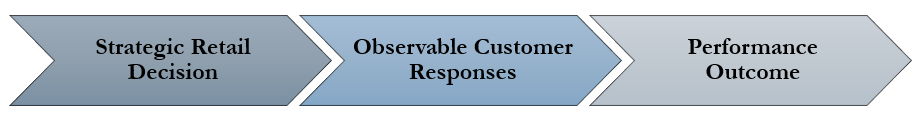
\includegraphics[width=1.02\textwidth]{chapter2_flow}
	\end{figure}
    
This structure applies across all four studies in the thesis. Each study investigates how a particular strategic action alters the customer decision-making context, and how that in turn affects performance outcomes such as sales, profitability, customer retention, and platform-based responses. While the empirical analyses focus on observable customer responses, the theoretical domains reviewed in this chapter provide guidance for interpreting the mechanisms that may underlie these responses. Because the analyses rely primarily on aggregated behavioral data, the intermediate decision processes of individual consumers cannot be directly observed but are instead inferred through theory and prior research (\cite{Hanssens2016-aa}). Table~\ref{tab:theory_overview} summarizes the conceptual focus of each study.

\begin{table}[!htbp]
\centering
\begin{tabular}{p{0.4cm} p{1.9cm} p{3.2cm} p{3.6cm} p{1.5cm}}
\hline
\textbf{Study} & \textbf{Strategic retail decision} & \textbf{Theoretical domains} & \textbf{Observable customer response: Key mechanism} & \textbf{Performance outcome} \\
\hline

1 & Setting price for multi-tier PLs across formats 
& Pricing across store formats; private label strategy 
& Purchase decision: Customers compare relative prices across PL tiers and perceive value differently 
& Sales, profits \\
\hline

2 & Adjusting regular price or offering promotions across formats 
& Pricing across store formats; reference price effects and price framing 
& Purchase decision: Customers perceive changes in regular price and discounts differently 
& Sales \\
\hline

3 & Channel introduction 
& Multichannel retailing; shopping utility and digital complementarity 
& Purchase decision: Customers, through changes that may not persist over time, adjust purchasing behavior after adopting the online channel 
& Category purchases, revenues \\
\hline

4 & Management of product exposure on digital platforms 
& Platform economy: Consumer behavior on digital platforms 
& Following decision: Customers have limited attention and need to choose certain contents to fit with their current situations 
& Platform-based responses (e.g., playlist followers) \\

\hline
\end{tabular}
\caption{Summary of Theoretical Domains and Empirical Focus Across Studies}
\label{tab:theory_overview}
\end{table}

This framework connects strategic retail actions, customer responses, and performance outcomes. Since these responses are context-dependent, empirical investigation helps quantify how the effects of strategies vary across contexts. Across the domains examined, the studies demonstrate how theoretical insights concerning (e.g.) reference price effects, shopping utility maximization, and platform economy provide a basis for interpreting observable customer responses. These insights provide explanations for why customer responses differ across contexts and how they translate into specific performance outcomes. Moreover, because theory can yield conflicting expectations across contexts, empirical analysis is important for assessing which explanations are more consistent with the data. Taken together, theory and empirics are closely linked: theory guides what to measure and examine while empirical evidence validates and refines theoretical relationships. 

%%%%%%%%%%%%%%%%%%%%%%%%%%%%%%%%%%%%%%%%%%%%%%%%%%%%%%%%%%%%%%%%%%%%%%%%%%%%%%%%%%%%%%%
% CHAPTER 3
\chapter[Data and Methodology]{Data and Methodology}\label{chap:datamethod} % 
This chapter outlines the empirical strategies used across the four studies in this thesis. It demonstrates how established empirical techniques are applied to different retail settings to examine the effects of strategic decisions on customer behavior and performance outcomes. Studies 1–3 rely on transaction-level data from a grocery retailer loyalty program; Study 4 uses publicly available data from the Spotify music streaming platform. Across these contexts, quantitative modeling approaches are designed to quantify how strategic retail decisions influence customer behavior and resulting performance outcomes. Table~\ref{tab:empirical_overview} provides a summary of the four empirical studies, including context, data source, its coverage, method, and level of analysis for performance outcomes. Each section then describes the research setting, data and sample construction, modeling approach, and limitations related to both data and modeling choices.

\begin{table}[htbp]
\centering
\begin{tabular}{p{0.5cm} p{1.3cm} p{2cm} p{2.8cm} p{3.4cm} p{1.3cm}}
\hline
\textbf{Study} & \textbf{Context} & \textbf{Data source} & \textbf{Coverage} & \textbf{Method} & \textbf{Level of analysis} \\
\hline

1 & Multiformat retailing 
& Retailer scanner data from loyalty program 
& 135,776 shopping trips over five selected product categories based on 4,921 customers 
& Error-correction model of sales response with price elasticity estimation and subsequent profit elasticity 
& Weekly brand sales \\
\hline

2 & Multiformat retailing 
& Retailer scanner data from loyalty program 
& 897,743 shopping trips from 5,468 customers 
& Two-stage approach: Price elasticity estimation followed by moderator analysis 
& Weekly brand sales \\
\hline

3 & Multichannel retailing 
& Retailer scanner data from loyalty program 
& 116,982 shopping trips across 578 households (147 of which adopt an online channel) 
& Propensity score matching combined with difference-in-differences estimation 
& Weekly customer purchases \\
\hline

4 & Digital platforms 
& Spotify playlist API and web-scraped data 
& 39,918 playlists with 49 consecutive weeks of follower data 
& Playlist-level unit fixed effects panel regression 
& Weekly playlist followers \\

\hline
\end{tabular}
\caption{Overview of empirical contexts, data, and methods across studies}
\label{tab:empirical_overview}
\end{table}

\section{Multiformat Retailing (Studies 1 and 2)}
The first two empirical studies are situated within the context of multiformat grocery retailing. They examine how pricing strategies perform, across different store formats, for one multi-format retailer. Despite belonging to the same retail chain, different formats cater to distinct shopping goals and create a unique context to explore customer responses to pricing decisions across different physical stores.

The data comes from the loyalty program of a major grocery retailer that operates in three store formats: hypermarkets, supermarkets, and convenience stores. From large-format stores catering to stock-up trips to medium-sized stores serving regular household needs and small outlets focused on immediacy and proximity, these formats differ substantially in size, assortment, and price positioning. Because shopping missions, basket sizes, time constraints, and assortment breadth systematically vary across these formats, customers are likely to respond differently to regular prices and promotions. For example, price discounts may be more salient for large, planned baskets at hypermarkets than for quick, convenience-driven trips at small stores. Promotional campaigns are coordinated centrally, while individual store managers retain flexibility in setting regular prices based on local market conditions. Taken as a whole, the situation reflects a multi-format strategy that combines service-oriented and price-competitive elements. Rather than following a strict everyday-low-price policy, the retailer maintains competitive regular prices but also relies on centrally coordinated promotions. This strategy is consistent with a hybrid or moderated hi–lo pricing format that lies between pure everyday-low-price and pure hi–lo in grocery retailing. The dataset includes detailed transaction-level records for approximately 5,500 customers over 153 consecutive weeks (2014–2016), covering around 900,000 shopping trips. Each record contains product-level information, including brand, category, regular price, promotional discount, and quantity purchased. This level of granularity allows for detailed measurement of customer behavior and pricing outcomes. From this dataset, study-specific samples are selected based on the requirements of each empirical design, resulting in differences in sample size and composition between Studies 1 and 2 (see Table~\ref{tab:empirical_overview}).

To evaluate how pricing strategies affect sales and profitability across physical store formats, the first two studies model customer responses using aggregated brand-level sales data. Aggregate sales response models are commonly used in retail pricing research because pricing decisions are typically implemented at the brand or category level rather than at the individual-customer level. Using brand-week panels therefore aligns the empirical model with the level at which retailers observe performance and make pricing decisions. Compared with individual-level choice models, this approach also reduces computational complexity while still capturing meaningful variation in customer responses to prices and promotions across store formats (\cite{Pauwels2007-ky,Datta2022-fz}). Thus, the unit of analysis of these studies is at the brand-week level, aggregated from transaction data, allowing the studies to quantify market-level customer response without relying on individual-level behavioral tracking. This approach is especially suitable for retailer-facing questions, such as whether specific pricing strategies improve sales or profitability across different retail formats.

To align with this modeling approach, the two studies leverage the same dataset to construct comparable brand-level sales panels across the three formats. The analysis focuses on the three store formats belonging to the same retail chain, located in the same area, for the purpose of ensuring the consistency and comparability of formats. To avoid biases due to assortment variation, products were selected based on consistent availability (a) across all three formats and (b) throughout the observation period, with an emphasis on frequently purchased brands. To ensure that any observed pricing effects were not confounded by size-based price differences, only items with standardized package sizes were retained. This approach mitigates the risk that format-based variation in sales is driven by differences in what is stocked, rather than by how customers respond to pricing.

In the first study, the focus is on profit-oriented evaluation of regular price setting for multi-tier PLs. The modeling follows a multi-step regression framework. First, price elasticities are estimated for each PL tier and format using observed variation in prices paid over time. These elasticity estimates are then combined with cost and price data to calculate contribution margins and profit effects. This two-part approach enables direct assessment of which tier–format combinations are most profitable, offering actionable insights for PL portfolio management (e.g., \cite{Geyskens2010-bx,Keller2020-so,ter-Braak2013-uq}).

In the second study, the focus shifts to how reference prices and discount framing affect sales across store formats. The study uses a two-stage regression design: the first stage estimates brand-level sales responsiveness to regular prices and promotions, and the second stage tests how these elasticities are moderated by brand characteristics, category type, and store format. This allows for identification of conditions under which either regular price changes or promotional discounts are more effective with respect to brand and category factors (e.g., \cite{Datta2022-fz,Haans2011-cv,Pauwels2007-ky}).

Both studies apply a sales response modeling framework (e.g., \cite{Pauwels2007-ky}), capturing how changes in price influence weekly sales volumes. An error correction specification is used because it allows the model to separate immediate demand reactions from longer-run equilibrium adjustments, which is particularly important when prices and promotions vary frequently across weeks. To mitigate endogeneity concerns, both models incorporate a set of control variables and fixed effects. These include brand fixed effects, time dummies, and category-level controls that help account for unobserved factors such as brand popularity, demand seasonality, and promotional cycles (\cite{Datta2022-fz}).

This modeling strategy offers several advantages. First, it mirrors managerial practice, where performance metrics like sales and margins are typically monitored at the weekly brand or category level (\cite{Widdecke2022-xo}). Second, by aggregating across customers, the models avoid the need for individual-level tracking (which is often unavailable in practice) while still revealing meaningful market-level behavioral responses. Third, the multi-step and multi-stage design enables a clear separation between estimating price elasticity and translating those effects into strategic insights about pricing, promotions, and profitability across brands, categories and formats.

While the dataset focuses on loyalty card holders from a single retail chain, it offers a high degree of consistency and detail, allowing precise observation of behavioral and sales dynamics over time within a stable customer base. Several limitations should however be acknowledged. First, the data do not capture purchases made at competing retailers; this may limit the generalizability of findings beyond the focal chain. Second, the analysis focuses on products consistently available across formats and time, enhancing comparability but possibly excluding niche or newly introduced items that could behave differently. Third, as the data reflect pricing and assortment decisions within one retailer’s organizational structure, some format-specific effects may be influenced by chain-level strategies that are not directly observable. In addition, the aggregate structure cannot capture within-brand heterogeneity in customer responses—for example, how different shopper segments may react to a given promotion (\cite{Ailawadi2004-ig, Geyskens2010-bx}). Furthermore, observed price variation is not randomly assigned and may reflect broader retailer strategy, so caution is required in interpreting causal claims (\cite{Bijmolt2005-kg, Datta2022-fz}). Despite these limitations, the combination of careful sample construction, consistent product selection, and inclusion of fixed effects for products, time, and store formats helps mitigate potential confounds from unobserved heterogeneity. This provides a reliable basis for assessing how pricing strategies influence performance across store formats.

\section{Multichannel Retailing (Study 3)}
The third empirical study, focusing on how customer purchase behavior evolves following the introduction of an online shopping channel, is set in the context of multichannel grocery retailing. Like the previous studies, it relies on transaction data from the retailer’s loyalty program, but it shifts the focus from store-format pricing to customer-level behavioral changes following online channel adoption. This setting provides a quasi-experimental setting to examine long-term shifts in behavior among customers who adopt (i.e., start using) the new channel, particularly whether online channel adoption leads to incremental revenue or simply redistributes spending across formats. \footnote{According to \textcite{Goldfarb2022-jt},
Quasi-experiment refers to the use of an experimental mode of analysis and interpretation to data sets where the data-generating process is not itself intentionally experimental (Campbell 1965). Instead, quasi-experimental research uses variation that occurs without experimental intervention but is nonetheless exogenous to the particular research setting.
}

The data come from the loyalty program of the same grocery retailer assessed in Studies 1 and 2, covering a four-year period that spans both pre- and post-introduction periods of the online channel. The online channel was introduced in late 2015, and this retailer was the only grocery chain in the region offering such an option at the time. This exclusivity minimizes competitive interference and enhances the internal validity of observed behavioral changes. The dataset combines two consecutive panels (October 2014–November 2016 and August 2017–July 2019) and tracks 578 households (147 of which adopt the online channel) across 116,982 shopping trips and roughly 1.75 million purchased products. The dataset includes customer-level purchase histories across both online and offline purchases, allowing for precise tracking of when each customer began using the online channel and how their purchasing patterns changed over time. Each transaction contains information on date, product category, quantity, spending, and purchase channel.

To identify the causal effect of online channel adoption on purchasing behavior, the study employs customer-level panel modeling techniques based on propensity score matching (PSM) and difference-in-differences (DiD) estimation. This approach is appropriate because online channel adoption is a voluntary decision rather than a randomized treatment. Propensity score matching, to reduce observable selection bias, first constructs comparable groups of adopters and non-adopters based on pre-adoption shopping behavior. Difference-in-differences estimation then exploits the panel structure of the data to compare behavioral changes before and after adoption at the customer level, thus helping isolate the causal impact of channel adoption from common time trends (\cite{Boehm2008-it, Campo2015-pt}).

To align with this modeling approach, the study leverages the loyalty data’s panel structure to track individual customers before and after the online channel introduction. Customers who adopted the online channel are compared against those who never adopted it throughout the observation window. This structure allows for the separation of pre-existing differences from actual behavioral shifts following adoption, thereby mitigating potential endogeneity concerns. By observing a panel of customers across a multi-year window (covering the before and after of the online channel’s introduction), the study captures longitudinal changes in behavior that follow the introduction and adoption of this new shopping format (\cite{Avery2012-ex,Bilgicer2015-ng}). This quasi-experimental setting allows the model to distinguish between behavioral changes caused by adoption versus those driven by general time trends or unobserved customer characteristics (\cite{Li2015-tq}).

This modeling strategy offers several advantages. First, it allows for customer-level inference, capturing the heterogeneity in how individuals respond to additional format adoption (\cite{Kushwaha2013-iu}). Second, the panel structure enables robust within-customer comparisons, reducing bias from unobserved time-invariant traits such as household size or income (\cite{Konus2008-mp}). Third, the combination of PSM and DiD mitigate self-selection bias by ensuring that adopters and non-adopters are comparable based on observable characteristics before the channel was introduced (\cite{Li2015-tq}), while DiD specifically controls for time-invariant unobservables and shared temporal trends.

While the dataset offers a unique opportunity to study an effect of online channel adoption on customer purchase behaviors, several limitations should be noted. First, although the retailer was the sole provider of online grocery shopping at the time of online channel introduction, competing retailers began offering similar services toward the end of the observation period; these are not explicitly accounted for. Second, because purchasing activity varies across customers, the ability to model detailed temporal dynamics (e.g., behavioral changes after one, two, or three years of adoption) is limited. Third, as the data reflect the early phase of adoption, the number of online users is relatively small and likely skewed toward early adopters, which may affect generalizability. In addition, DiD relies on the parallel trends assumption, that in the absence of treatment, adopters and non-adopters would have followed similar trajectories over time (\cite{Li2023-ho}). This assumption cannot be directly tested and may become less plausible as the post-adoption period extends. While matching helps improve group comparability, the use of proxies such as diaper purchases and store distance may not fully capture deeper household characteristics. Furthermore, DiD is less effective when treatment timing varies across individuals, or when adoption reflects structural changes in customer behavior that evolve gradually rather than in discrete shifts (\cite{Roth2023-xe}). Despite these limitations, matching and DiD allow comparison of purchasing behavior between adopters and non-adopters over time. The combined use provides a transparent and meaningfully practical basis for assessing how online channel adoption affects customer behavior over time.

\section{Digital Platforms (Study 4)}

The fourth empirical study is situated in the context of digital platforms, where customer behavior can be largely shaped by platform structures and mechanisms such as algorithmic curation and editorial decisions. Because these systems determine what users see and engage with, they influence which participants on the platform gain attention, or traffic. In such environments, potential external disruptions like the COVID-19 pandemic can alter user behavior at scale, raising questions about how users interact with content shift after the onset of such an event. Unlike the other studies, which rely on retailer loyalty data, this one uses publicly available platform data to examine observable user responses in a digital marketplace.

The data are extracted from publicly available sources related to Spotify, one of the world’s leading music streaming platforms. The dataset combines two primary sources. First, playlist-level follower data was obtained from Chartmetric, a commercial analytics provider that aggregates historical data from Spotify’s web API. This dataset includes weekly follower counts, curator type (e.g., Spotify-owned, label-affiliated, or independent), and content features such as the share of tracks from major labels and average track popularity. Second, data from Every Noise at Once is used to identify weekly instances of playlists featured on that platform, which is equivalent to platform-driven promotion that increases visibility. By integrating this information, the analysis distinguishes between follower growth (arising from organic user responses) and platform-driven exposure. The starting dataset from Chartmetric included over 1.2 million playlists. From this, playlists were filtered in stages: first, only those with sufficient data continuity were retained, and those lacking key variables, such as curator type, genre, or content attributes, were excluded. The final sample consists of 39,918 active playlists with 49 consecutive weeks of data spanning October 2019 to October 2020, thus covering periods before and after the pandemic was declared.

To examine changes in user responses on the platform, the study models playlist follower growth using fixed effects panel regression. Weekly follower changes serve as a proxy for aggregate observable user responses. A fixed effects panel specification is used because playlists differ systematically in their baseline popularity, genre, and curator characteristics. By controlling for these time-invariant playlist attributes, the model isolates within-playlist changes in follower growth over time (\cite{Papies2022-ln}).

To align with this modeling approach, the dataset is structured as a playlist-level panel observed over time, thus allowing each playlist to be tracked before and after the pandemic declaration. Each playlist serves as an observation unit, with time-varying attributes such as follower counts, content composition, curator type, and promotional exposure. The resulting dataset enables comparison of changes in follower growth within the same playlist over time, rather than across inherently different playlists. Key independent variables include playlist curator type, content composition, and weekly indicators of platform-driven promotion (i.e., Search Page featuring).

This modeling strategy offers several advantages. First, the playlist-level panel allows for detailed tracking of engagement changes across a broad sample of Spotify playlists. Second, the fixed effects specification accounts for unobserved heterogeneity at the playlist level, such as theme, brand strength, or historical growth patterns, which supports more credible within-playlist comparisons over time. Third, the inclusion of week fixed effects helps control for seasonality and platform-wide shifts in user activity, allowing changes in follower growth to be more closely associated with the pandemic period rather than general time trends.

First among limitations to be noted with regard to the fourth study, the dataset captures publicly observable playlist-level metrics such as follower counts rather than individual user behavior, and this leads to limited insights concerning the micro-level drivers of engagement. Second, the influence of Spotify’s algorithmic or editorial decisions is not directly observable and must be inferred from the featuring data. Third, follower growth serves as a proxy for user response and does not capture listening intensity or financial outcomes. In addition, the fixed effects model might be better suited for estimating large, persistent changes in engagement rather than subtle or short-lived shifts. As such, for smaller effects (particularly those limited to a subset of playlists or time periods) it may be harder to isolate the effect with certainty and subject to attenuation. Finally, even with week fixed effects, any unobserved time-varying shocks that affect playlists differently may not be fully captured by the model structure. Despite these constraints, the panel structure and fixed effects specification allow for consistent measurement of changes in user responses over time, particularly in response to large-scale external disruptions such as the pandemic (\cite{Denk2022-rt,Sim2022-ns}).

 

%%%%%%%%%%%%%%%%%%%%%%%%%%%%%%%%%%%%%%%%%%%%%%%%%%%%%%%%%%%%%%%%%%%%%%%%%%%%%%%%%%%%%%%
% CHAPTER 4
\chapter[Empirical Studies]{Empirical Studies}\label{chap:study} % 
This chapter presents the four empirical studies. The following sections detail each study’s motivation, empirical design, key findings, and contributions. While each study targets a specific decision and context, they collectively illustrate how data-driven approaches, grounded in consumer behavior theory, can be used to assess the effectiveness of strategies across formats, channels, and digital platforms.

\section{Study 1}

\textbf{From Price to Profit: Multi-Tier Private Label Response Across Retail Formats}

\noindent
\textit{Authorship:} Tanetpong Choungprayoon (Stockholm School of Economics)

\noindent
\textit{Status:} Working paper. An earlier draft was presented at the 53rd Annual Conference of the European Marketing Academy in 2024.

\noindent
***

Retailers increasingly use PLs not only to enhance margins but also to differentiate their assortments and target heterogeneous customer segments across store formats. Multi-tier PL strategies (typically comprising value, standard, and premium tiers) enable retailers to address heterogeneous customer preferences and strengthen store identity. However, the effectiveness of these tiers depends on store context. The same price change may have different consequences across formats that differ in assortment and in the shopping missions and customer expectations they facilitate. This study examines how price elasticities of multi-tier PLs (and the resulting profit effects of pricing decisions) vary across hypermarkets, supermarkets, and convenience stores.

Previous research has established the growing importance of PLs and the benefits of tiered strategies (\cite{Ailawadi2008-zy,Geyskens2010-bx}), but empirical evidence on how these effects differ across retail formats remains limited (\cite{Keller2022-tz}). While prior work shows that customer price responsiveness can vary across store formats (e.g.,\cite{Haans2011-cv}), existing studies often treat PL pricing as uniform, overlooking the possibility that store format moderates both customer price sensitivity and cross-tier interactions. This study addresses the research gap by quantifying how pricing responses differ across tiers and formats, and by linking these responses to profit outcomes.

To analyze the effectiveness of PL pricing across tiers and formats, the study employs a two-stage modeling framework linking demand responses to profitability outcomes. The specification captures the interdependence among PL tiers by incorporating cross-price effects across tiers. First, a sales response model is estimated using an error correction specification that includes both own-price and cross-price effects across PL tiers. This structure allows the model to capture within-category substitution and cannibalization effects that arise when price changes in (e.g.) the value tier influence sales in (e.g.) the premium tier. Short-term elasticities are normalized to enable comparison across categories and formats, and are used to simulate expected changes in sales volumes under different pricing conditions. Second, a profits-response model is estimated, also in error correction form. The model incorporates predicted changes in sales (derived from the sales response model) as key inputs, linking quantity adjustments back to pricing decisions. This step allows the estimation of format- and tier-specific profit elasticities, reflecting how price changes translate into bottom-line outcomes under real-world cannibalization and substitution dynamics. Both models include controls for seasonality, store-week effects, and endogeneity (via Gaussian copula terms), ensuring robustness of the estimates.

The findings reveal three key insights. First, customer price responsiveness varies significantly across formats, even within the same PL tier and category. Second, cross-tier pricing effects are nontrivial, meaning that offering a discount on a value tier product may boost volume for that tier but reduce sales in adjacent tiers, especially in formats with constrained assortments. Third, profitability outcomes are highly format-contingent. While premium PLs tend to be less elastic overall, their margin benefits depend on format-specific volume dynamics and price sensitivity.


\section{Study 2}
\textbf{Regular Prices vs. Discounts: How Pricing
Strategies Perform Across Store Formats}

\noindent
\textit{Authorship:} Tanetpong Choungprayoon (Stockholm School of Economics), Rickard Sandberg (Stockholm School of Economics), and Sara Rosengren (Stockholm School of Economics)

\noindent
\textit{Status:} Working paper. An earlier draft was presented at the 51st Annual Conference of the European Marketing Academy in 2022.

\noindent
***

Retailers frequently rely on two key pricing tactics to drive sales: adjustments to regular prices and the use of promotional discounts (i.e., temporary price cuts). While both tools can influence customer behavior, they are not equivalent in either perception or outcome. This study examines how regular price changes and promotional discounts differentially affect sales across retail formats within the same grocery chain. The analysis builds on the idea that shopping goals vary across formats, even for the same customers, yielding diverging responses to price cues.

Existing literature has highlighted the psychological distinctions between regular prices and promotional discounts (e.g., \cite{DelVecchio2006-xp,Shankar1996-kq}). While prior research has explored how customers respond to price changes, fewer studies have empirically disentangled the effects of regular price changes and promotional discounts across different store formats within the same retail chain. This study leverages an important feature of the empirical setting: promotional campaigns are largely centrally coordinated, while individual store managers retain flexibility in setting regular prices.

The analysis is based on data from a grocery retailer. It draws on three stores, one representing each format: a hypermarket, a supermarket, and a convenience store. All three are located in the same geographic area to minimize demographic and regional variation. Categories, products, and brands are selected based on consistency of purchase across format and time, allowing reliable cross-format comparison of price responsiveness. In the first stage of the analysis, we estimate regular price and discount elasticities for brand sales using an error-correction model of sales response following \textcite{Pauwels2007-ky}, with controls for category traffic and trip types (major, fill-in, and unplanned). These controls help account for differences in shopping behavior across formats. In the second stage, we regress the estimated elasticities on brand- and category-level attributes such as discount frequency, discount depth, PL status, storability, and category competitiveness to examine how these characteristics explain variation in pricing effectiveness across formats.

The findings reveal three key insights. First, regular price elasticities are negative across all store formats, with the strongest magnitude in hypermarkets and the weakest in convenience stores. Discount elasticities are also highest in hypermarkets, followed by supermarkets, indicating stronger responsiveness to promotional pricing in larger formats. Second, product characteristics matter: categories that are storable or impulsive exhibit higher discount sensitivity, while brands with deeper and more frequent promotions tend to experience greater discount elasticity. Third, depending on format and positioning, PLs show distinct patterns in their responses to price cues.



\section{Study 3}

\textbf{The Long-Term Effects of Online Channel Adoption in Grocery Retailing}
\noindent
\textit{Authorship:} Tanetpong Choungprayoon (Stockholm School of Economics), Emelie Fröberg (Stockholm School of Economics), and Sara Rosengren (Stockholm School of Economics))

\noindent
\textit{Status:} The current draft was initially given a “reject and resubmit” decision and was later rejected by the \textit{Journal of Retailing}.

\noindent
***

The introduction of digital channels has reshaped grocery retailing by offering consumers greater flexibility while posing new challenges for retailers. Many studies have examined who adopts online grocery shopping and why, but fewer have explored how purchasing behavior evolves in the long term after adoption. This study investigates how customer purchase behavior changes after the introduction of an online channel, and whether such adoption leads to sustained revenue growth for the retailer.

Previous research shows that adding new channels can benefit retailers because multichannel customers often spend more than single-channel shoppers (\cite{Ansari2008-qz,Kumar2005-nn}). Yet these effects may vary across product categories (\cite{Kushwaha2013-iu}) and depend on the specific benefits that the new channel provides (\cite{Bell2018-yn,Melis2016-mf}). In grocery retailing, habitual purchasing and the mix of hedonic and functional goods make long-term behavioral shifts particularly uncertain. Studies suggest that online channels enhance shopping utility for certain categories (e.g., bulky or heavy items that are convenient to order online) but reduce it for products requiring physical inspection or freshness evaluation (\cite{Campo2015-pt,Campo2020-xu}). However, less is known about whether these category-specific effects persist or attenuate over time.

To address this gap, our study builds on the theory of shopping utility maximization, which posits that consumers choose purchase patterns that yield the highest total utility. Shopping utility comprises two components: acquisition utility, referring to the benefits of the products offered (e.g., price and assortment), and transaction utility, referring to the convenience and effort associated with obtaining them (e.g., ordering and delivery). In this context, the retailer offered identical prices and assortments across channels, keeping acquisition utility constant. Differences in transaction utility therefore drive observed behavioral changes. The framework links three levels of outcomes: (a) category-level effects driven by perceived online ordering convenience, delivery convenience, and ordering risk; (b) customer-level effects on shopping frequency and monetary value; (c) retailer-level effects on total revenue.

The empirical analysis uses loyalty card data from a Nordic grocery retailer that launched an online channel in late 2015. The sample follows 578 households over a five-year period, including both adopters and non-adopters of the online channel. To identify long-term effects, the study applies a DiD design combined with PSM. It compares purchasing behavior before and after adoption while controlling for self-selection and customer heterogeneity.

The results show that the long-term effects of adoption are consistent with our theoretical framework. Customers who adopted the online channel spent more in product categories that offered high delivery convenience (e.g., bulky or heavy products) and spent less in sensory categories associated with higher perceived online purchase risk. In contrast, purchases of categories associated with online ordering convenience showed no significant long-term change. At the customer level, shopping frequency remained broadly stable while the average monetary value per purchase increased over time. These changes led to higher total expenditure among adopters, indicating higher long-term revenue for the retailer.

This study extends previous research on multichannel retailing by providing empirical evidence on the long-term effects of online channel adoption across category, customer, and retailer outcomes. It also illustrates how a framework based on shopping utility maximization can help retailers analyze influences of digital channel adoption on customer value over time.



\section{Study 4}
\textbf{How Did COVID-19 Affect Playlist Followers on Spotify?}

\noindent
\textit{Authorship:} Tanetpong Choungprayoon (Stockholm School of Economics), Hannes Datta (Tilburg University), and Max Pacheli (Tilburg University)

\noindent
\textit{Status:} Unpublished manuscript. An earlier draft was presented at Economics of the Music Industry in 2022.

\noindent
***

The COVID-19 pandemic reshaped how music was consumed and discovered, particularly on digital platforms where playlists have a central role in promoting track consumption. This study investigates how follower dynamics on Spotify playlists changed during the pandemic. The focus is on curator identity, playlist popularity, and share of major-label tracks. The purpose is to assess how an external disruption affected engagement and the distribution of visibility among stakeholders operating within a platform-controlled environment.

Previous research has shown that playlists have a central role in shaping music discovery and consumption on streaming platforms (\cite{Aguiar2018-wt,Datta2018-xz}). However, most existing evidence comes from periods of normal platform activity, and this limits understanding of how engagement patterns shift when external shocks disrupt user routines. Our study addresses the limit by examining how playlist follower growth responded to the pandemic. It offers insight on how platform exposure and curator outcomes evolved under disruption.

The study investigates these issues through four empirical questions related to overall follower changes, playlist popularity, curator type, and share of major-label tracks within playlists. Together, these questions assess whether engagement during the pandemic became (a) more concentrated among dominant stakeholders or (b) more broadly distributed across the platform.

The empirical analysis uses playlist-level data from Spotify, collected through third-party sources including Chartmetric for follower information and Every Noise at Once for playlist featuring indicators. The final sample, covering periods before and after the pandemic was declared, includes 39,918 active playlists tracked weekly from October 2019 to October 2020. Focusing on within-playlist variation, the empirical strategy employs a unit fixed effects model to estimate how playlist followers changed before and after the pandemic onset. This approach controls for persistent playlist characteristics (e.g., genre, theme, long-run popularity) while measuring the effect of time-varying pandemic indicators. Three complementary measures are used: a binary indicator for the pandemic declaration, a country-weighted government Stringency Index capturing the intensity of restrictions, and a country-weighted measure of residential mobility capturing changes in time spent at home.

The study also examines heterogeneous effects across playlists. Playlists are categorized into five popularity tiers based on follower percentiles, allowing the analysis to compare highly popular “superstar” playlists with mid-tail and long-tail playlists. In addition, playlists are classified according to curator type (including Spotify, major labels, independent labels, artists, professional curators, and users). Finally, the analysis considers the share of tracks from major record labels within each playlist to evaluate whether established industry content influenced follower growth during the pandemic.

The results show that there was no significant change in average follower growth following the pandemic declaration. However, an increase in follower growth when government restrictions intensified and users spent more time at home suggests that playlist engagement responded more to behavioral changes than to the declaration itself. The effects also differed across playlists. Mid-tail and long-tail playlists experienced relatively stronger growth compared to the most popular superstar playlists, indicating a broader distribution of engagement across content. Spotify-curated playlists were more resilient than those curated by other stakeholders, and (particularly among mid-tail and long-tail playlists) they showed stronger follower growth. Playlists with higher shares of major-label tracks showed some positive association with follower growth, but this effect was relatively small once track-level popularity was taken into account.

These findings demonstrate how large-scale disruptions can reshape engagement patterns on digital platforms. During the pandemic, follower growth became less concentrated among the most popular playlists, yet platform-curated playlists maintained a strong position within the ecosystem. The results highlight the role of platform governance, curator resources, and content composition in shaping visibility and engagement on streaming platforms across periods of external disruption.




 

%%%%%%%%%%%%%%%%%%%%%%%%%%%%%%%%%%%%%%%%%%%%%%%%%%%%%%%%%%%%%%%%%%%%%%%%%%%%%%%%%%%%%%%
% CHAPTER 5
\chapter[Discussion and Future Directions]{Discussion and Future Directions}\label{chap:discussion} % 
In this final chapter, I step back from the specifics of each study to reflect more broadly on what the thesis contributes. The specific contribution from each separate study is outlined in the corresponding article \textbf{(See Appendix)}. The sections that follow are organized into four sections describing theoretical contributions, managerial implications, methodological notes, and limitations (with directions for future research). Each section connects insights across the empirical studies to identify recurring patterns and broader lessons that extend beyond the individual analyses. Across these sections, the chapter provides an integrated synthesis of the thesis’s main contributions and outlines directions for future research.

\section{Theoretical Contributions}

This thesis contributes to marketing and retail theory by demonstrating how large-scale behavioral data, when analyzed through established consumer behavior theories, can be used to examine how strategic decisions relate to customer responses across different retail settings. Following a consumer-based strategy perspective, which emphasizes the use of insights from customer behavior to inform strategic decisions ((\cite{Hamilton2016-ca}), the studies treat observable customer responses as the unit of analysis. These responses provide a behavioral basis for assessing how strategic decisions play out across contexts, rather than interpreting outcomes in isolation.

First, this thesis highlights the importance of retail context when evaluating the strategies’ effectiveness. Across Studies 1–4, results illustrate that customer responses to retail strategies are not consistent across formats, brands, channels, and platform participants. Studies 1 and 2 show that, even within the same retailer, the impact of pricing strategies and discounts for PL products cannot be generalized. Price elasticities and profit outcomes differ systematically by store format, PL tier, and product category. These findings align with prior research on multiformat retailing and PLs (e.g., \cite{Geyskens2010-bx,Haans2011-cv}), and with broader evidence on variations in marketing mix across formats (\cite{Wichmann2021-vm}). They also suggest that performance should not be evaluated using aggregated effects alone, but must account for differences across context, brand, and assortment. Study 4 extends this context principle to digital platforms to reveal that Spotify’s playlist follower dynamics during the pandemic did not follow uniform patterns but differed by curator type and content composition. It further shows that, consistent with broader platform dynamics, external shocks can shift visibility and outcomes unevenly across platform participants (\cite{Wichmann2022-gq}).

Second, the studies jointly demonstrate that customer responses help explain how strategic actions translate into observable outcomes. Rather than presenting outcomes without explanation, each study links strategic actions (e.g., pricing, channel introduction, and platform management) to customer responses in purchasing or platform interaction. For example, Study 3 draws on shopping utility maximization to explain why online channel introduction for a grocery context altered the mix and monetary value of purchases over time. The study expands on work by \textcite{Campo2015-pt} and \textcite{Melis2016-mf}, and it aligns with recent evidence on household adaptation to economic pressures and category-level adjustments (\cite{Scholdra2022-rp}). It shows that long-term revenue changes are driven by persistent shifts in the categories from which customers purchase. In particular, customers increase spending in categories with higher online delivery convenience, and this leads to higher value per visit over time. Study 4, in turn, shows that customer behavior on digital platforms reflects broader shifts in daily routines during COVID-19. As time spent at home increased, users adjusted their listening behavior, leading to changes in how attention was distributed across playlists. These patterns are more clearly understood when observed behavior is interpreted in relation to external conditions.

Third, the thesis refines existing knowledge on pricing and channel strategies. Through comparison of regular price changes, temporary discounts, and PL tiers, in Studies 1 and 2 the findings show that neither price nor discount elasticity is consistent across products and store formats. For example, Study 2 shows that discount responsiveness is stronger in hypermarkets than in smaller formats. Study 1 further shows that profitability differs across PL tiers depending on store format. These results build on previous findings (e.g., \cite{Ailawadi2006-he,Shankar1996-kq,Widdecke2022-xo}) and highlight that the effectiveness of pricing strategies depends on both store format and assortment structure. Study 3 similarly shows that the effects of online channel adoption on long-term value are not uniform but dependent on how customers adjust their purchasing behavior over time.

Last, the thesis emphasizes both the value and the limits of data-driven approaches. By leveraging unique retailer and platform datasets that directly connect strategy to observed behavior, the studies show that insights do not come from data volume alone but from how data are interpreted. Common generalizations, such as the belief that discounting always increases sales, or that online channels always add value, are shown to depend on context. The thesis therefore substantiates calls for theory-driven, context-aware analytics (\cite{Dekimpe2020-bh}), echoing similar arguments for more adaptive, context-specific decisions on marketing mix (\cite{Wichmann2021-vm}). It suggests a model for future research that balances prediction with explanation.

\section{Managerial Implications}

Many of the findings in this thesis are not new to practitioners. Price and discounting are not the same thing. Store formats influence how customers behave. Platforms tend to favor their own content. However, the issue is that these insights are not often reflected in how decisions are actually implemented or evaluated in practice. As noted by \textcite{McKinsey-Company2021-wc}, performance reports often aggregate prices and promotions under a single pricing which obscures their distinct effects. Store formats have traditionally been treated primarily as alternative offering channels, not as distinct behavioral contexts. Recent industry reports (e.g., \cite{Accenture2024-vg,Bain-Company2025-hz}) suggest that retailers are beginning to rethink this view.

The contribution of this thesis is therefore not to introduce new ideas but to quantify and structurally outline what is already known. By testing these differences across formats, categories, and time, the studies show where common assumptions hold and where they do not. In particular, they show that applying the same strategy across contexts can lead to very different outcomes. This is consistent with prior work showing that managerial insights are more useful when grounded in real-world data and linked to practical decisions (\cite{Schauerte2023-dn}).

Take, for instance, the idea that deep discounts drive sales. This is generally true, but the effect could depend on format, product category, and timing. Studies 1 and 2 show that profit gains from price increases on budget PLs hold in hypermarkets but not in supermarkets. Promotion fatigue also varies across categories, and customers’ past exposure to discounts reduces discounts’ future effectiveness. These findings are not new, but they are rarely quantified or compared across formats, categories, and customer groups. The key implication is not simply that discounts work or that formats matter, but that applying the same pricing approach across products, formats, or customer groups can lead to suboptimal outcomes. Managers therefore need to be more precise in how they frame and evaluate pricing decisions.

In place of such broad advice as “be agile” or “embrace personalization” (advice often found in industry reports; e.g., \cite{Accenture2024-vg,McKinsey-Company2019-cx}), by quantifying effects across formats, categories, and time this thesis shows where differences actually matter. The findings are based on observed customer behavior in real empirical settings, and they demonstrate that practical improvements come from making more precise and structured use of existing data.

This thesis also challenges the common assumption that more data will necessarily improve decision-making. Retailers and platforms already have access to large amounts of data, yet the main challenge often lies in how that data is interpreted. Across the studies, better insights are not driven by larger datasets but by framing decisions through consumer behavior theory (e.g., in terms of utility, perceived value, or platform structure). In this sense, theory can serve as a practical tool for interpreting observed patterns, especially when data are noisy or incomplete. Understanding customer behavior—grasping why customers switch channels, respond to price changes, or interact with content—may be more transferable than relying solely on additional data or tools. This does not imply that data are unimportant, but it does imply that more data alone may not always lead to better decisions.

Further, this thesis contributes is its attention to time. In practice, for example in campaign planning, time is often treated as an operational detail rather than as part of how decisions are made. Across the four studies, the results show that the duration of effects, their persistence over time, is just as important as the effects themselves. Study 1 distinguishes between short- and long-run price responses. Study 3 tracks how customer behavior changes after online channel adoption and which of these changes persist over time. Study 4 examines how follower patterns shift in response to a system-wide disruption. These analyses focus on more concrete questions: what persists, for whom, and for how long? By treating time as part of the analysis, not only as a reporting interval, the thesis highlights how effects can build, fade, or change over time.

Finally, while the studies are empirically grounded in grocery retail and music streaming, their implications extend beyond these settings. The findings from multiformat pricing and multichannel allocation are relevant for other frequently purchased categories such as health, household goods, or personal care. Similarly, the results on platform behavior apply not only to Spotify but also to retail environments that manage digital visibility through search results, home page placements, and recommendation systems. What matters is not the domain but how format, price, assortment, and customer decision-making interact. These interactions are not industry-specific; they arise whenever businesses manage what customers see and how they choose across formats and channels.

\section{Methodological Notes}

Throughout this thesis, theory serves as a guide in shaping the empirical approach. The choice of variables, model structures, and empirical specifications are all grounded in prior research to ensure that the results speak to meaningful constructs in retail strategy and consumer behavior. In particular, each study connects theoretical findings to measurable and observable outcomes (e.g., how price changes affect sales and profit, how channel adoption changes purchasing behavior, or how platform exposure relates to follower dynamics). This helps ensure that the empirical results remain connected to meaningful managerial questions.

A recurring methodological consideration across the studies is the use of panel data structures that support analysis of customer behaviors’ change over time. This thesis uses three complementary empirical strategies depending on the level of decision: error-correction modeling (ECM) for pricing responses, DiD for channel adoption, and panel fixed effects models for platform behavior. These approaches are used not only to control for unobserved differences but also to capture how effects evolve over time. Panel data enables examination of not just whether a strategic action has an effect but how that effect may change over time. Since the research questions emphasize both immediate and longer-term responses to retail decisions, temporal dynamics are treated in the course of the analysis. In Studies 1 and 2, ECM separates short-term effects from longer-term adjustments in sales and profits (\cite{Pauwels2007-ky}). Study 3, comparing pre- and post-periods between matched customer groups, uses a difference-in-difference design to track sustained behavioral changes after digital channel adoption (\cite{Golder2022-bo}). Study 4 applies fixed effects panel models with time controls to isolate change while accounting for shocks related to the COVID-19 pandemic. Across all four studies, these methods allow the analyses to identify whether effects are short-lived or persistent, and how they develop over time. This is consistent with prior research emphasizing that consumer behavior is dynamic and should be analyzed over time (\cite{Zhang2021-os}).

Another important aspect of the methodological approach is the use of real-world data from retailers and digital platforms. This thesis prioritizes high external validity by studying actual observed customer behavior in real decision environments. Across all studies, efforts were made to account for unobserved heterogeneity, to control for confounding factors, and to use robust estimation techniques. The first study applies ECM to estimate both short- and long-term price effects across PL tiers and formats; it thereby links sales responses to profit outcomes. The second study uses a sequential regression design to isolate differential effects of regular pricing and discounts while accounting for brand- and category-level moderators. The third study employs a difference-in-differences design with PSM to estimate long-term behavioral changes following online channel adoption. The fourth study, leveraging government restriction indices and mobility data to contextualize pandemic effects uses a unit fixed effects panel model to assess changes in playlist followers over time. These designs reflect the shared goal of extracting credible insights from observational data while acknowledging its boundaries. This design aligns with recent calls for an empirics-first approach, where theory generation is grounded in the systematic analysis of real-world behavioral data, not imposed a priori (\cite{Golder2022-bo}).

What ties the empirical studies together is the effort to link observed behavioral outcomes such as purchasing responses, channel adoption, and follower changes to broader retailer-level outcomes. This approach reflects the belief that meaningful analysis is derived not from statistical complexity alone but from efforts to build bridges between components of a problem (\cite{Leeflang2014-fs}). For example, in the pricing studies, the analysis moves beyond elasticity to consider profit response and substitution across PL tiers. In the online channel adoption study, the analysis goes from product mix shifts to sustained revenue differences. In the platform study, follower changes are used as observable indicators of exposure and response. This ensures that the analysis remains relevant for understanding performance outcomes.

Finally, the studies follow a consistent structure from theory to empirical specification and interpretation. Each study starts from a theoretical framework to guide the choice of variables and model specification. The empirical results are then interpreted in light of these theoretical expectations. This structure helps maintain comparability across contexts, and it ensures that the analysis remains grounded in both theory and observed behavior. Using established methods with real-world data strengthens the validity of the results and supports their practical relevance.

\section{Limitations and Future Directions}

Like all empirical research, this thesis is shaped by constraints in data, scope, and method. Recognizing these limitations is important, not only for the validity of the current findings but also for guiding future research that builds on and improves them. While each empirical study has its own specific boundaries, several overarching themes emerge across the thesis. These include contextual scope, modeling constraints, and data design and inference.

All four studies are embedded in specific retail and platform environments. This fact strengthens internal validity but limits broader generalization. The pricing analyses (Studies 1 and 2) rely on data from a single Nordic grocery retailer where loyalty norms, assortment structures, and competitive intensity may differ from what is found in other markets. Similarly, while the online channel study (Study 3) is situated in an early-adoption setting, the platform analysis (Study 4) focuses on a single period of pandemic disruption. These contextual boundaries invite replication across other geographies, sectors, and timeframes to test the robustness of the patterns identified here. Future research could extend the framework to new categories or retail systems to examine whether the interaction between context, strategy, and consumer response persists under different market conditions (\cite{Gielens2019-si}).

A second set of limitations concerns the focus and operationalization of key constructs. The pricing studies isolate regular price and discount effects but do not include such other marketing instruments as in-store displays, advertising, and supplier promotions (\cite{Bijmolt2005-kg,Nijs2001-qq}). This simplification allows for clean estimation of price responsiveness but may understate the joint influence from other marketing actions. In the online channel study, the quasi-experimental design captures behavioral outcomes following adoption, but it simplifies the adoption process itself. Channel adoption is modeled as a discrete event by abstracting from managerial interventions (e.g., communication campaigns or delivery incentives) that might influence both the likelihood and intensity of adoption. Moreover, the focus on grocery purchases, with their unique delivery constraints and purchase rhythms, limits the generalizability of behavioral patterns to other product or service categories (\cite{Campo2020-xu,Kushwaha2013-iu}). Finally, the platform study uses playlist followers as a proxy for engagement, an approach that captures visibility and attention but not actual consumption or revenue outcomes. Together, these modeling constraints highlight a trade-off between analytical clarity and strategic completeness. Future research should address this gap by integrating richer managerial, cost, and behavioral data to achieve a more comprehensive understanding of performance outcomes.

A final limitation stems from reliance on observational data. The quasi-experimental design of Study 3 and the fixed effects approach in Study 4 strengthen causal interpretation but cannot fully eliminate unobserved heterogeneity or selection bias (\cite{Goldfarb2022-jt}). Early adopters may differ systematically from non-adopters in ways that are difficult to observe, from digital literacy to risk tolerance and time constraints, which can influence both their likelihood of adoption and their subsequent purchasing behavior (\cite{Avery2012-ex,Li2015-tq,Rietveld2018-ay}). Similarly, playlist performance may reflect algorithmic or editorial choices that, made by the platform, are not visible to researchers and make it challenging to disentangle organic audience behavior from platform-driven amplification. Across all four studies, the reliance on observational data brings the typical trade-offs of real-world research: high external validity but limited causal precision. Future research could combine field experiments, A/B testing, and simulation-based methods with observational data to more directly examine the underlying behavioral processes that cannot be observed in the current data. Integrating survey-based or qualitative insights could also reveal psychological mechanisms behind the behavioral patterns observed.

Overall, the limitations identified in this thesis highlight opportunities for future research. Addressing these through broader contexts, richer data, and complementary methods would help strengthen and extend the insights developed here.
 

%%%%%%%%%%%%%%%%%%%%%%%%%%%%%%%%%%%%%%%%%%%%%%%%%%%%%%%%%%%%%%%%%%%%%%%%%%%%%%%%%%%%%%%
% EPILOGUE
\chapter*{Epilogue}
\addcontentsline{toc}{chapter}{Epilogue}
\markboth{Epilogue}{}

% --- Local figure numbering for Epilogue (safe, no appendix interference)
\setcounter{figure}{0}
\renewcommand{\thefigure}{E\arabic{figure}}

Having highlighted in Chapter \ref{chap:discussion} what this thesis contributes to theory, practice, and methodology, I cannot help but feel a little strange writing about such contributions as if they belonged in separate boxes. This reflection is not meant to be generalizable, and it would certainly fail an external validity test. Then again, it’s meant as reflection, not replication. I reflect that none of these insights came from pursuing any contribution in isolation. Over five years of sweat and tears, I realized that they came from a messy, nonlinear process. Sometimes they came accidentally, sometimes intentionally, but most of the time procedurally. This is because the process by which I arrived at the contributions was a process made up of cycles. The cycles involved understanding the data, making sense of them, recognizing limitations, building visual tools, refining models, and then interpreting the results and the story they seemed to tell.

To make sense of anything, I first had to understand the data—not just statistically, but structurally and contextually. What did each variable represent? What patterns were already there before I started drawing lines through the data or asking algorithms to discover them for me? What was missing, why, and what could be done about it? These questions became the starting point for every project. And just as much as theory guides analysis, the data often forced me to revisit assumptions and rethink the questions I was asking. Eventually, I learned to ask better questions, shifting from “Is this effect significant?” to “What does this tell us about how people behave (or don’t) in certain situations, and about how businesses respond?”

Throughout my studies, some of the most striking insights did not come from rigorous models or perfect specifications. And by striking, I don’t mean the most statistically robust. Those came later, after the models were built and the story had already been laid out. The real insights came while exploring data through interactive dashboards that I designed myself. They allowed me to visualize patterns, compare segments, and trace how key variables evolved over time through colors, shapes, and simple interactive elements such as filters and dropdowns. No hypothesis tests, no coefficients; just time series, simple cohort comparisons, and a thousand tabs open at once. 

These tools were not merely exploratory. They suggestively pointed toward observed patterns. They didn’t prove the patterns, and working with them was less about analyzing the data, more about narrating it, about trying to see where meaning might be hiding. It felt like holding a book of theory in the dark, with the dashboard offering just enough light to read a few lines at a time. Some might say it’s enough to read in the dark, if you just focus hard enough. Others might say it’s all about finding the light and seeing what appears. But I think I prefer a little light to guide the reading.

Looking back on this process, I have come to realize that research in the social sciences is not just about technical proficiency or theoretical advancement. It is about learning to navigate contradictions between theory and data, detail and direction, explanation and uncertainty. It is about knowing when to zoom in on a variable and when to step back and ask if that variable matters at all. The research I conducted became less a process of control and more a negotiation with the data, the related literature, and my own assumptions. And while some might prefer to treat assumptions as something objective or at least external to the researcher, I’ve learned that they are anything but. They shape what we see, what we ignore, and what we are willing to believe the data is telling us.

Part of the reason I came to see research this way is that this thesis took long enough for me to spend some time in industry. The more I moved between the two (full time at the bank and part time at the PhD office), the stranger it felt to hear people talk about academia versus industry as if they constituted different worlds. From my experience, the academic process is almost identical to the industry process. Both try to make sense of observed behavior, to predict outcomes and improve decisions, whether through behavioral explanations or algorithmic models. The only real difference is emphasis. Academia polishes its explanations until they are publishable. Industry polishes its tools until they are profitable. One asks what is going on and why. The other asks what to do next. Both chase relevance, each through a different lens: the microscope of academia and the binoculars of industry.

That said, I can’t resist a confession.

Sometimes I wonder if social science has (or will) become a full-blown circus of triviality. Everyone’s performing, juggling regressions, walking the tightrope of robustness checks, and pulling contributions out of hats. We spend years polishing results so safe, so painfully obvious, that any trace of something even slightly interesting is lost under layers of statistical rigor. Then comes the best part: we frame the findings in terms of what they add to the literature, even though it always remains the same literature, in the same journals, read by the same people. As if the point of research were not to understand the world but to impress insiders. The only real novelty? A new dataset, usually slightly bigger or slightly weirder than the last one. It is exhausting. We are rewarded for saying something new (not necessarily something true, and not always something useful). At times, I feel like we are just optimizing for clever footnotes on the margins of irrelevance.

But let’s not pretend industry isn’t running its own sideshow. If academia is a circus of triviality, then industry is a magic show of illusory certainty, of quick solutions pulled out of black box algorithms, of KPIs waved like proof of wisdom, of ambiguity made to disappear behind convincing tables and dashboards. Industry frames impact but fears uncertainty, celebrates innovation but avoids reflection. The costumes differ, but the performance is the same: a pursuit of efficiency over understanding, staged according to the same kind of instrumentalism.

And yet, I remain optimistic. Because the real value, I think, lies in the overlap. In realizing that research is not just about what practitioners can learn from us, but what we can learn from them. People in industry do not need to be told context matters; they live in it. They do not theorize about heterogeneity; they market to it. And maybe, just maybe, good research is not the kind that holds itself apart from practice. Maybe it’s the kind that builds practice from tools, constraints, and theory, lit by a dashboard like the one that sparked every idea in this thesis.


% --- Restore original figure numbering (important for appendix later)
\renewcommand{\thefigure}{\arabic{chapter}.\arabic{figure}}

% FULL THESIS REFERENCES
\cleardoublepage
\chapter*{References}\addcontentsline{toc}{chapter}{References}
\markboth{References}{}
\SSEprintbibliography{none}

%%%%%%%%%%%%%%%%%%%%%%%%%%%%%%%%%%%%%%%%%%%%%%%%%%%%%%%%%%%%%%%%%%%%%%%%%%%%%%%%%%%%%%%
% APPENDIX
\appendix

\chapter{From Price to Profit: Multi-Tier Private Label Response Across Retail Formats}
\label{app:article1}
\markboth{Article 1}{}

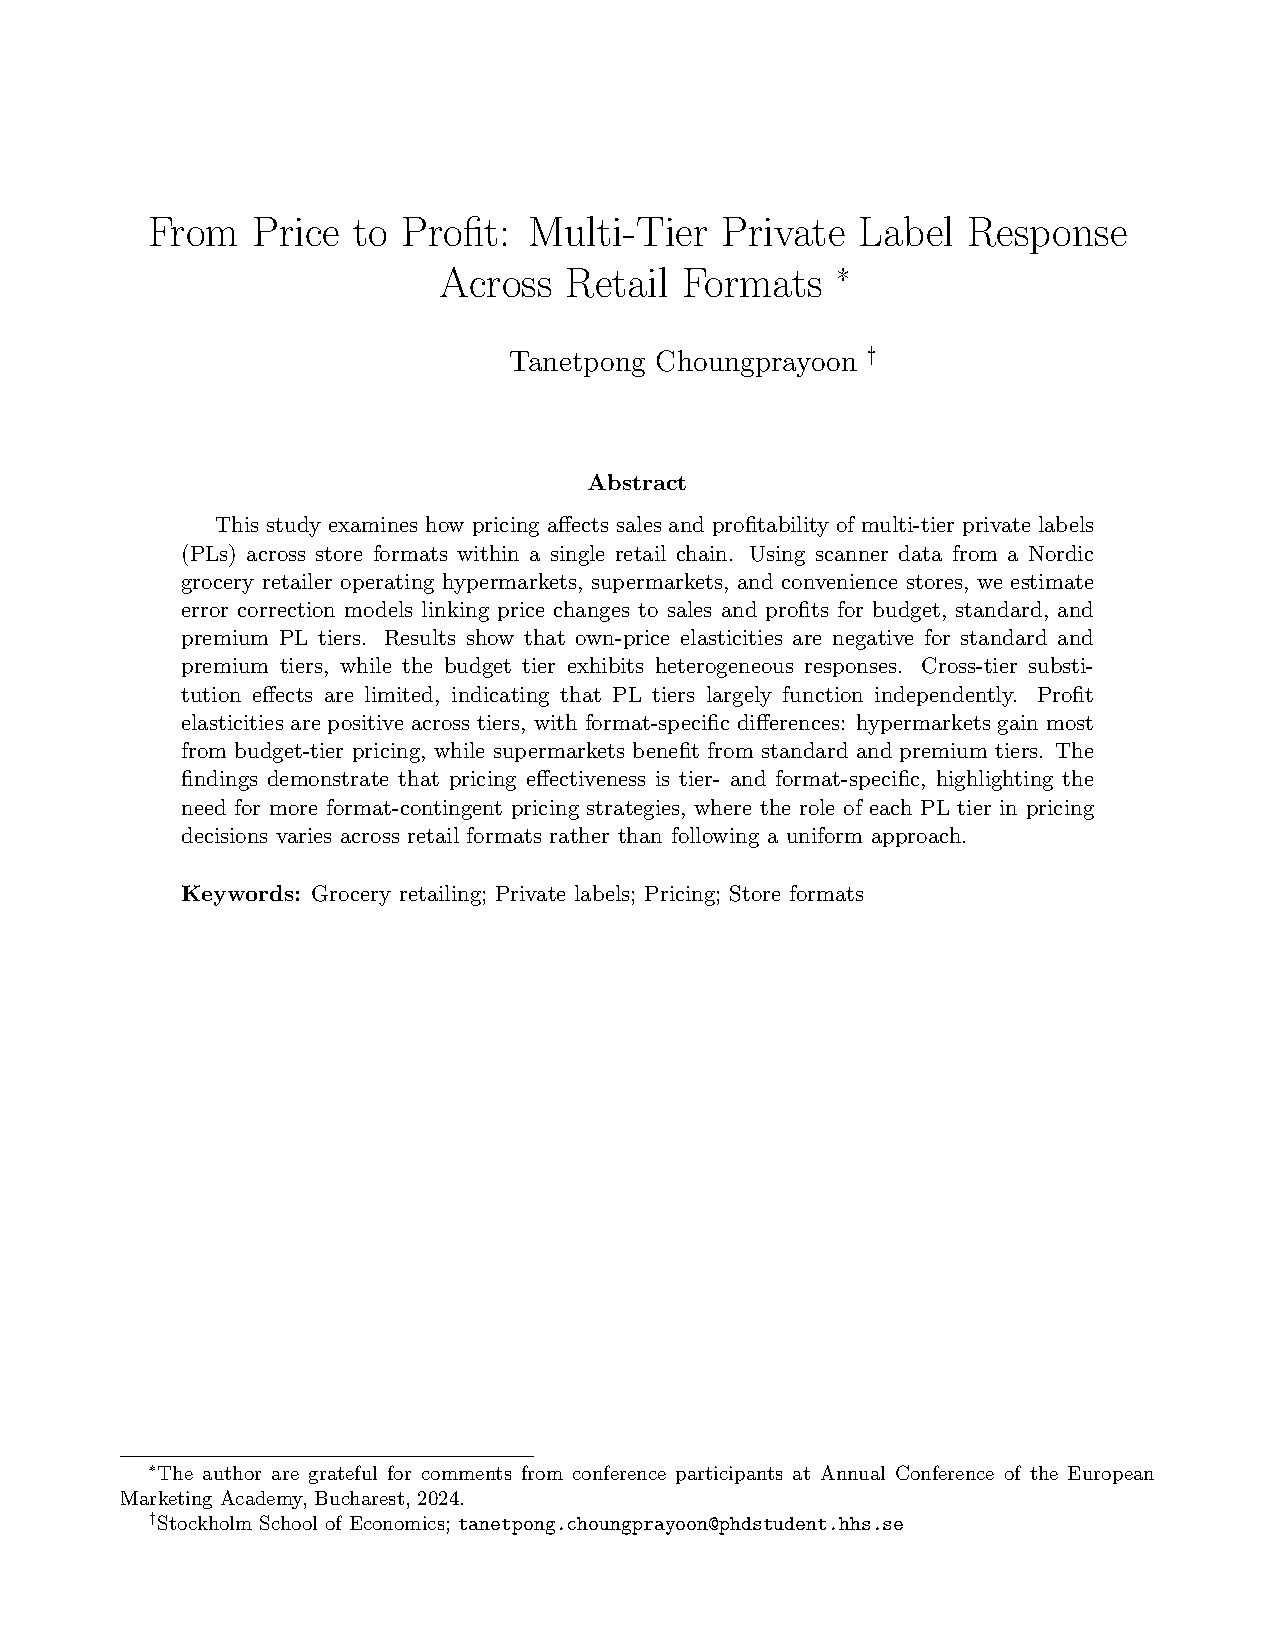
\includepdf[
  pages=-,
  pagecommand={\thispagestyle{ssethesis}},
]{chapters/article/article1.pdf}

\chapter{Regular Prices vs. Discounts: How Pricing Strategies Perform Across Store Formats}
\label{app:article2}
\markboth{Article 2}{}

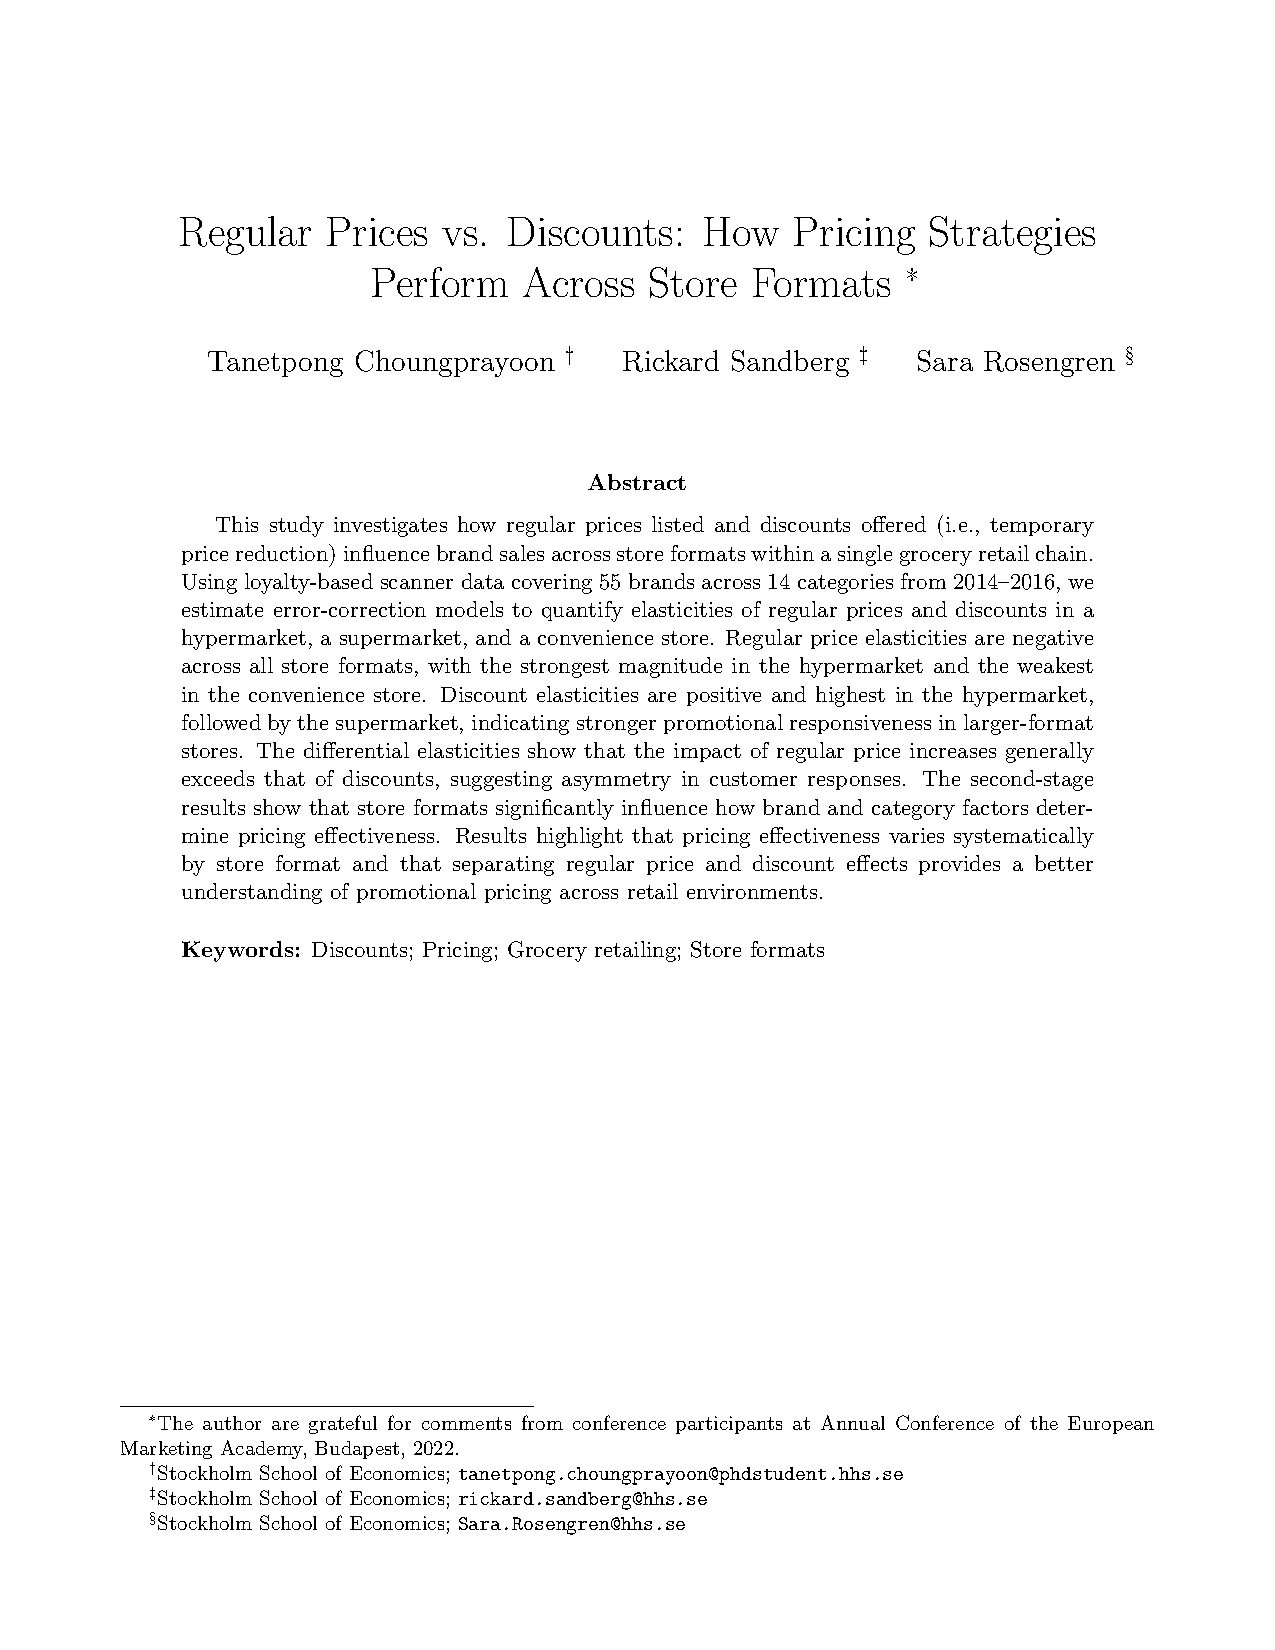
\includepdf[
  pages=-,
  pagecommand={\thispagestyle{ssethesis}},
]{chapters/article/article2.pdf}

\chapter{The Long-Term Effects of Online Channel Adoption in Grocery Retailing}
\label{app:article3}
\markboth{Article 3}{}

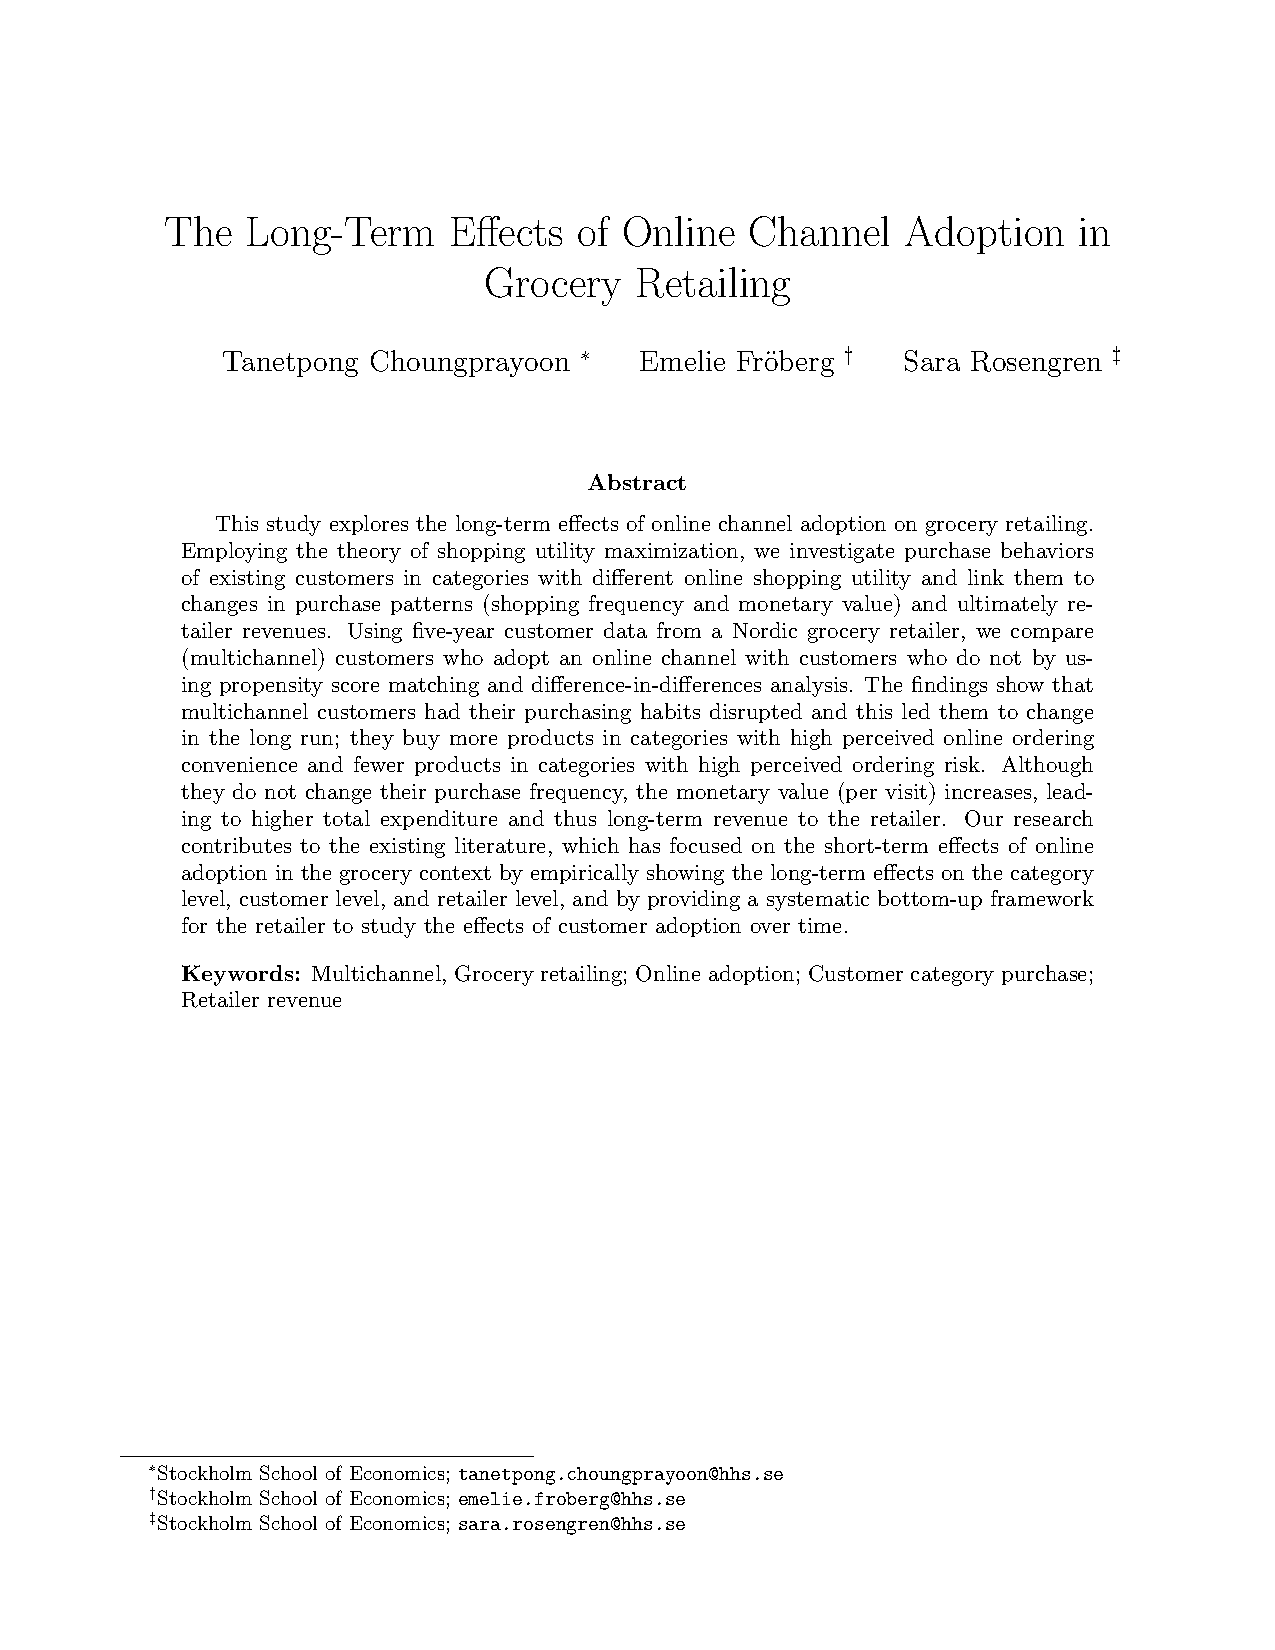
\includepdf[
  pages=-,
  pagecommand={\thispagestyle{ssethesis}},
]{chapters/article/article3.pdf}

\chapter{How Did COVID-19 Affect Playlist Followers on Spotify?}
\label{app:article4}
\markboth{Article 4}{}

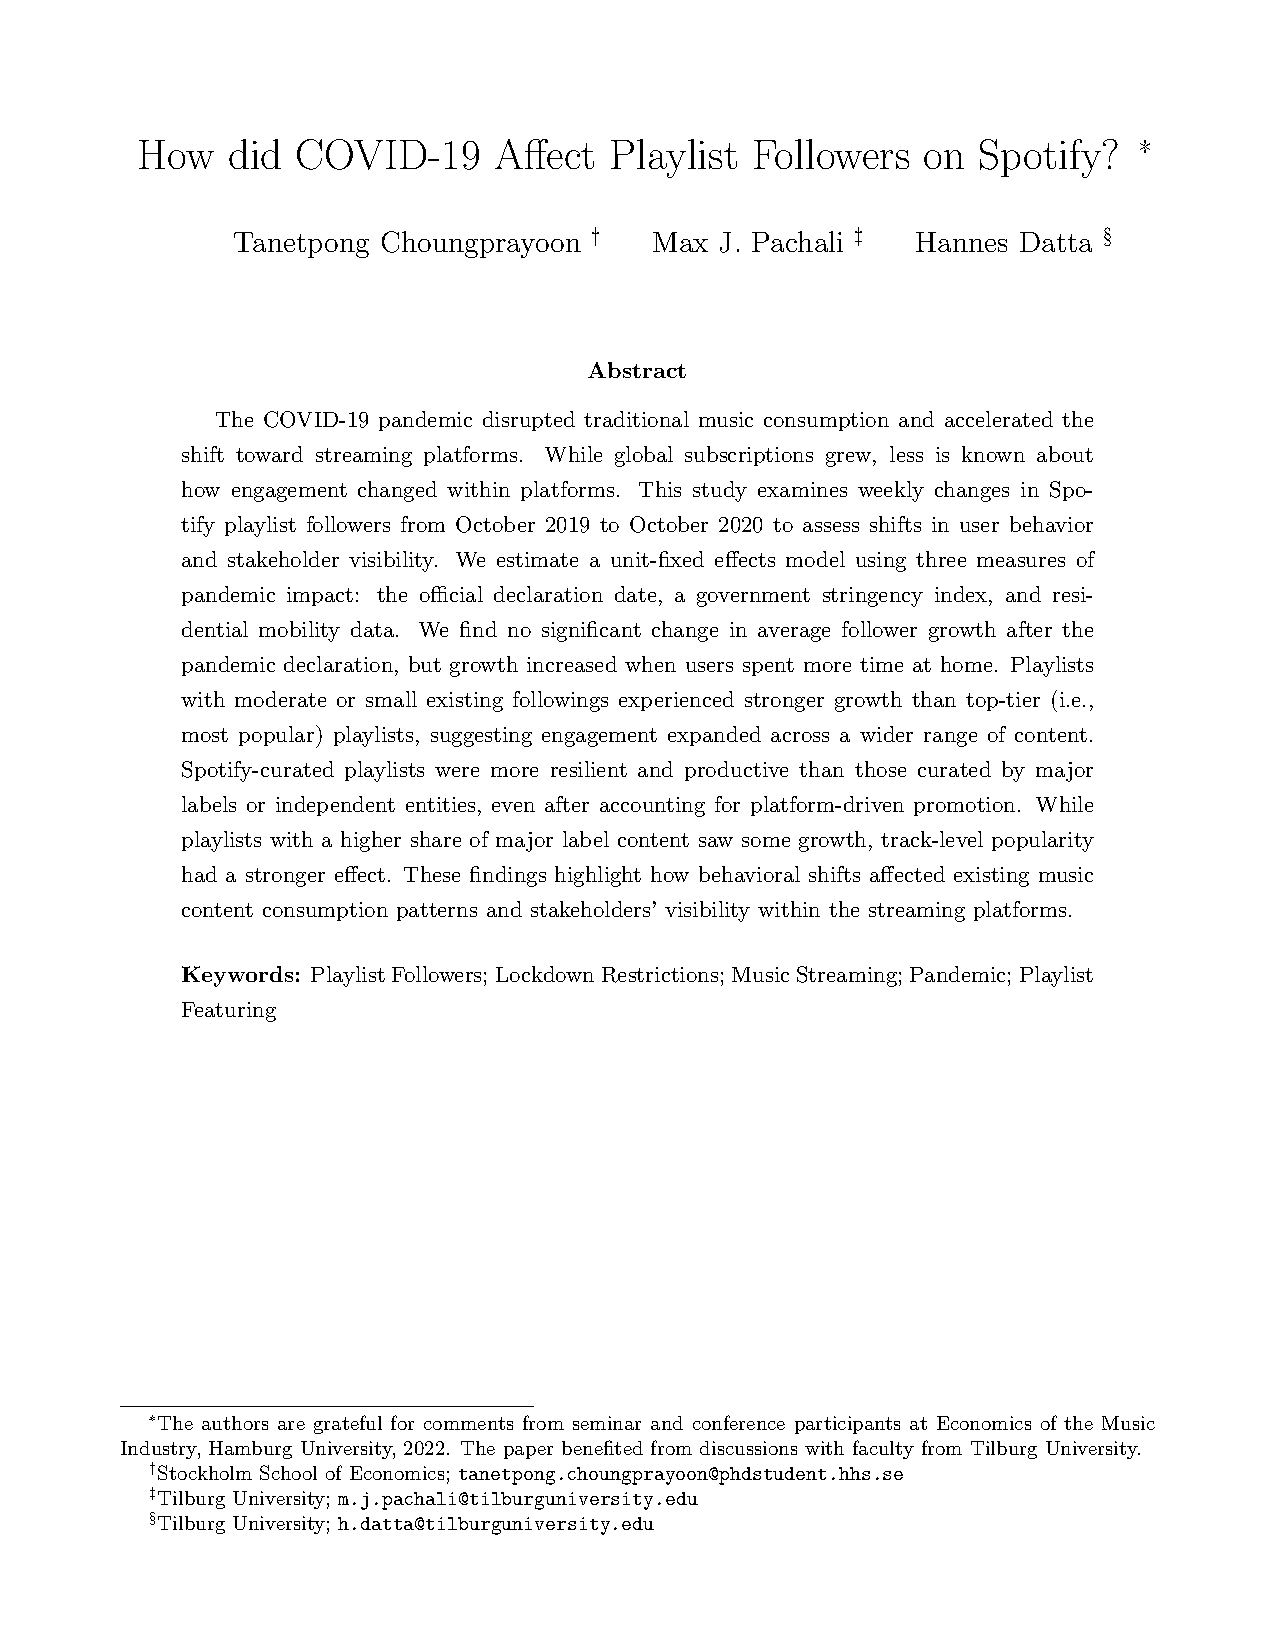
\includepdf[
  pages=-,
  pagecommand={\thispagestyle{ssethesis}},
]{chapters/article/article4.pdf}

\end{document}


%%%%%%%%%%%%%%%%%%%%%%%%%%%%%%%%%%%%%%%%%%%%%%%%%%%%%%%%%%%%%%%%%%%%%%%%%%%%%%%%%%%%%%%
% CHAPTER 1
\begin{refsection}
	\chapter[Introduction]{Title of Chapter~1: the subtitle is extremely long whereby the title must be shortened to fit in the Table of Contents and header}\label{chap:introduction} % The optional argument provides a shortened version of the title for the ToC and header
	% \chaptermark{Header title of Chapter~1} % Shorter version of the title for the header only
	{\large\centering\theauthor\par\vspace*{2\onelineskip}} % Author
	\begin{abstract}\input{chapters/chapter1/abstract}\end{abstract}%
	\blindfootnote{Who am I grateful to?}%
	\include{chapters/chapter1/mainmatter} % include puts clearpages around automatically
	\begin{subappendices}
		% "fake" new chapter to get the unnumbered chapter style for appendix (also does a cleardoublepage)
		\SSEfakechapter{\thechapter.A}{Appendix}%
		\input{chapters/chapter1/appendix} % need to use input to not clearpage
		\SSEfakechapter{\thechapter.B}{References}\SSEprintbibliography{none}
	\end{subappendices}
\end{refsection}

